\documentclass
[handout]
{beamer}
\usepackage{bm}
\usetheme{Malmoe}
\begin{document}
\title[Simulation]{Statistical Computing: Simulating Random Variables}
\date{May 24}
\author{Anastasios Panagiotelis / Feng Li}
\institute{Monash University / Central University of Finance and Economics}
\maketitle
\section{Motivation}
\begin{frame}{A mathematical  problem}
\begin{itemize}
\item Suppose the floor is covered in boards.  A needle is randomly dropped onto the floor.
\pause
\item What is the probability that the needle lies on a crack between the boards?
\pause
\item This problem was originally posed by Buffon.
\end{itemize}
\end{frame}
\begin{frame}{Buffon's needle}
\begin{center}
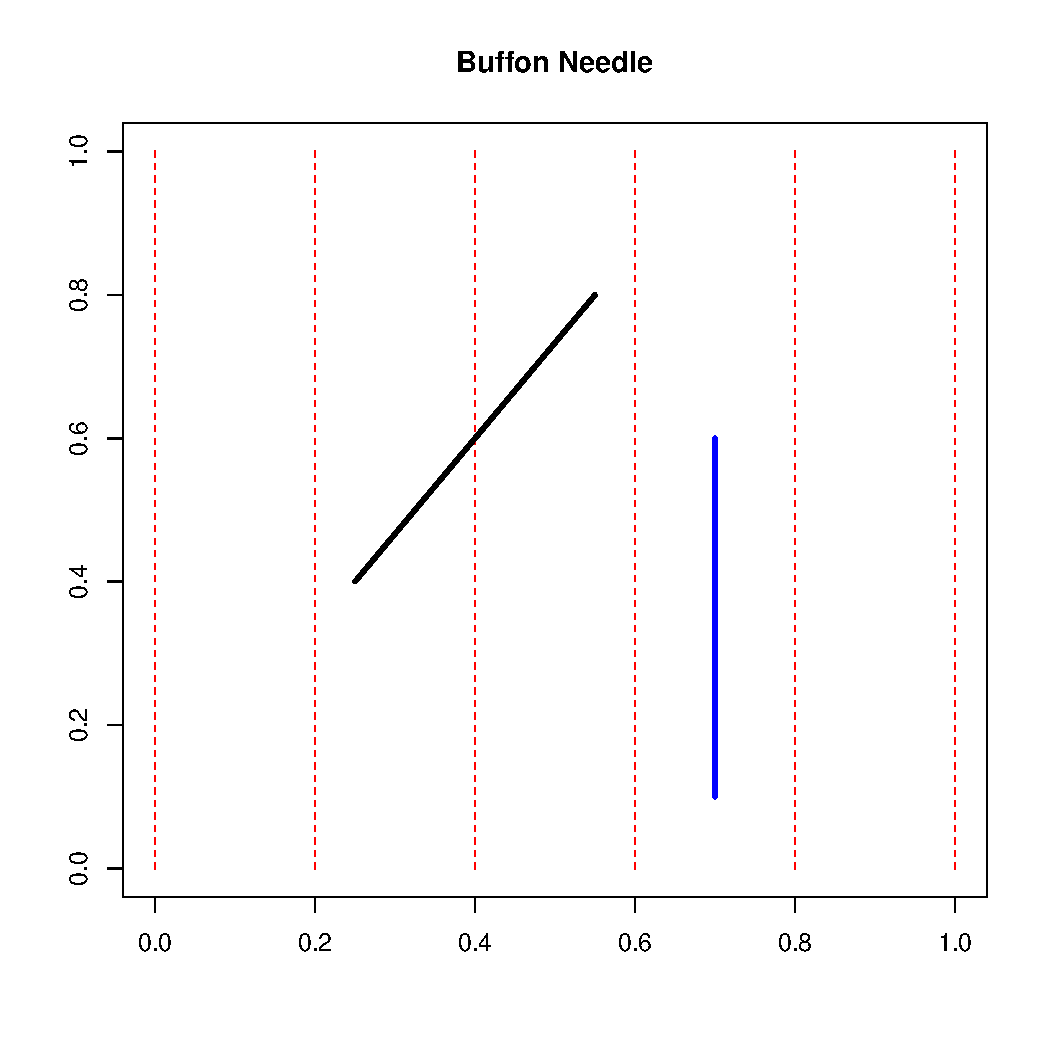
\includegraphics[height=7cm]{./Pics/buffonneedle.pdf}
\end{center}
\end{frame}
%\begin{frame}{Not this Buffon...}
%\begin{center}
%
\includegraphics[height=7cm]{./Pics/Gigi.jpg}
%\end{center}
%\end{frame}
%\begin{frame}{This Buffon}
%\begin{center}
%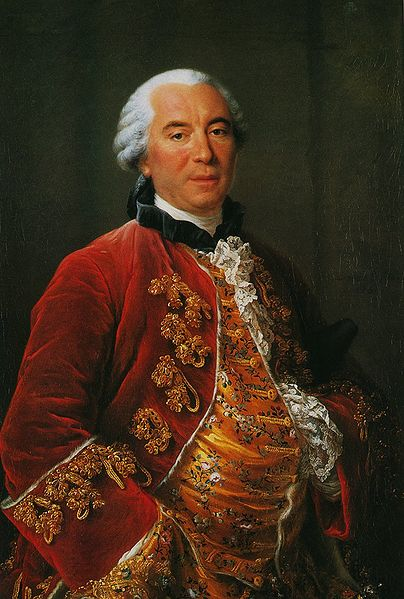
\includegraphics[height=7cm]{./Pics/Buffon.jpg}
%\end{center}
%\end{frame}
\begin{frame}{A difficult mathematical problem}
\begin{itemize}
\item This is a difficult problem to solve analytically
\pause
\item An easy way to solve the problem would be to actually drop many needles on the floor.
\pause
\item The number of needles that fall on a crack could be counted and divided by the total number of needles.
\pause
\item This task is too time consuming for a human, so perhaps a computer can do it instead...
\end{itemize}
\end{frame}
\begin{frame}{An retirement problem}
\begin{itemize}
\item Now consider an example from business and in particular actuarial studies.
\pause
\item Suppose that I am planning how much money I will keep for retirement.
\pause
\item I will invest some of my money in stocks, some in bonds and some in houses.
\end{itemize}
\end{frame}
\begin{frame}{Investment strategy}
\begin{itemize}
\item I spend half of my salary and invest the other half.
\pause
\item For the half I invest, 40\% is in stocks, 40\% is in houses and 20\% is in bonds.
\pause
\item If there is a year where the stock market crashes, the following year I invest 60\% in stocks, 20\%  in houses and 20\% in bonds.
\pause
\item When am 55 years old, I invest 20\% in stocks, 20\%  in houses and 60\% in bonds.
\pause
\item If I am 65 and still have less than \$200000, then I keep working for five more years.
\end{itemize}
\end{frame}
\begin{frame}{Probability Distribution of Investment}
\begin{itemize}
\item What is the probability distribution of the final value of my investment?
\pause
\item This is difficult to solve.
\pause
\item However, we may have a model to forecast the returns in stocks, housing and bonds.
\pause
\item If we simulate from these models, it is then easy to write a computer program that computes the final value of the investment.
\end{itemize}
\end{frame}
\begin{frame}{Monte Carlo}
\begin{itemize}
\item The idea of using computer simulation to solve difficult problems like these is known as the {\bf Monte Carlo} method
\pause
\item It is an extremely useful idea in economic, financial and business applications.
\pause
\item It is also a useful idea in {\bf statistical inference}.
\pause
\item In particular in the Bayesian paradigm, inference is based on the {\bf posterior distribution} of the parameters.
\end{itemize}
\end{frame}
\section{Direct Simulation}
\begin{frame}{Only need Uniform}
\begin{itemize}
\item Assume that we have a way to simulate from a uniform distribution between $0$ and $1$, $u\sim U(0,1)$ 
\pause
\item If this is available, it is possible to simulate many other probability distributions.
\pause
\item The most simple method is the {\bf Direct Method}
\end{itemize}
\end{frame}
\subsection{Discrete Case}
\begin{frame}{Discrete Case: Example 1}
\begin{itemize}
\item Assume that we want to simulate a binary variable $X$ with $\mbox{Pr}(X=0)=0.3$ and $\mbox{Pr}(X=1)=0.7$
\pause
\item Let $u\sim U(0,1)$.  Then the following rule can be used
\begin{equation}
x=\left\{\begin{array}{c}
0 \quad \mbox{if $u<0.3$}\\
1 \quad \mbox{if $u>0.3$}\\
\end{array}
\right.
\end{equation}
\pause
\item It is expected that if this is repeated many times 30\% $X=0$ and 70\% $X=1$
\end{itemize}
\end{frame}
\begin{frame}{Discrete Case: Example 2}
\begin{itemize}
\item Assume that we want to simulate a discrete variable $X$ with $\mbox{Pr}(X=0)=0.3$ and $\mbox{Pr}(X=1)=0.25$ and $\mbox{Pr}(X=2)=0.45$
\pause
\item Let $u\sim U(0,1)$.  Then the following rule can be used
\begin{equation}
x=\left\{\begin{array}{l}
0 \quad \mbox{if $u<0.3$}\\
1 \quad \mbox{if $0.3<u<0.55$}\\
2 \quad \mbox{if $u>0.55$}
\end{array}
\right.
\end{equation}
\pause
\item It is expected that if this is repeated many times, roughly 30\% $X=0$, 25\% $X=1$ and  45\% $X=2$
\end{itemize}
\end{frame}
\begin{frame}{Visualization: Example 1}
\begin{center}
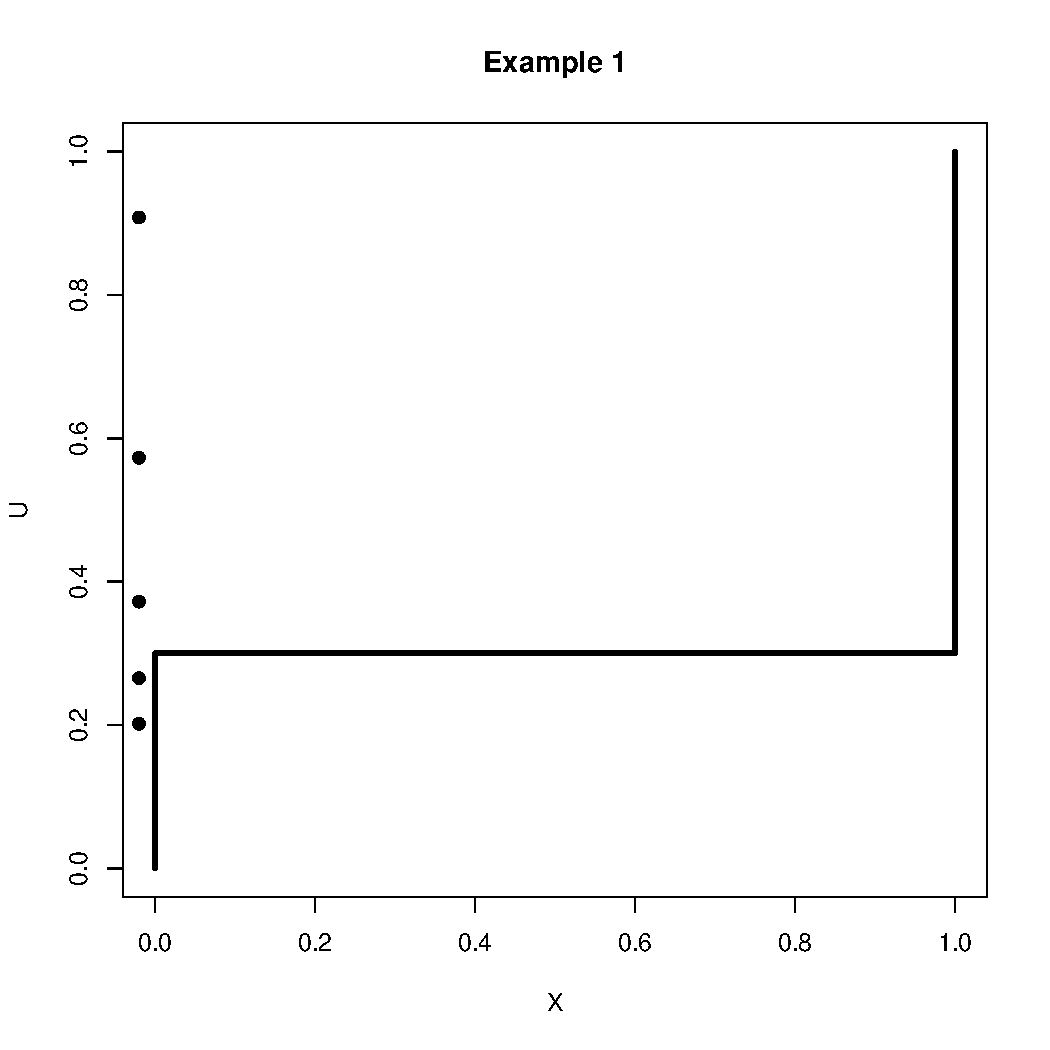
\includegraphics[height=7cm]{./Pics/d1p1.pdf}
\end{center}
\end{frame}
\begin{frame}{Visualization: Example 1}
\begin{center}
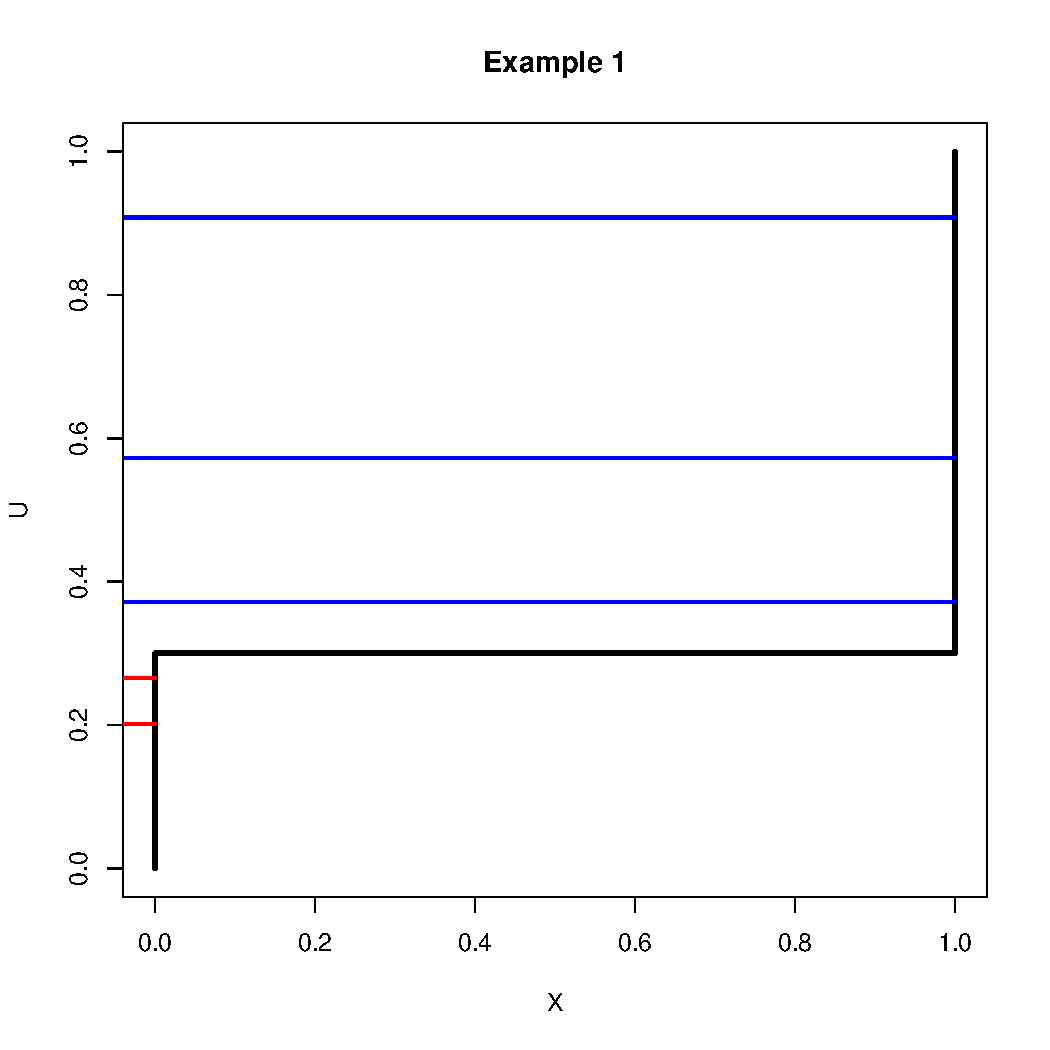
\includegraphics[height=7cm]{./Pics/d1p2.pdf}
\end{center}
\end{frame}
\begin{frame}{Visualization: Example 1}
\begin{center}
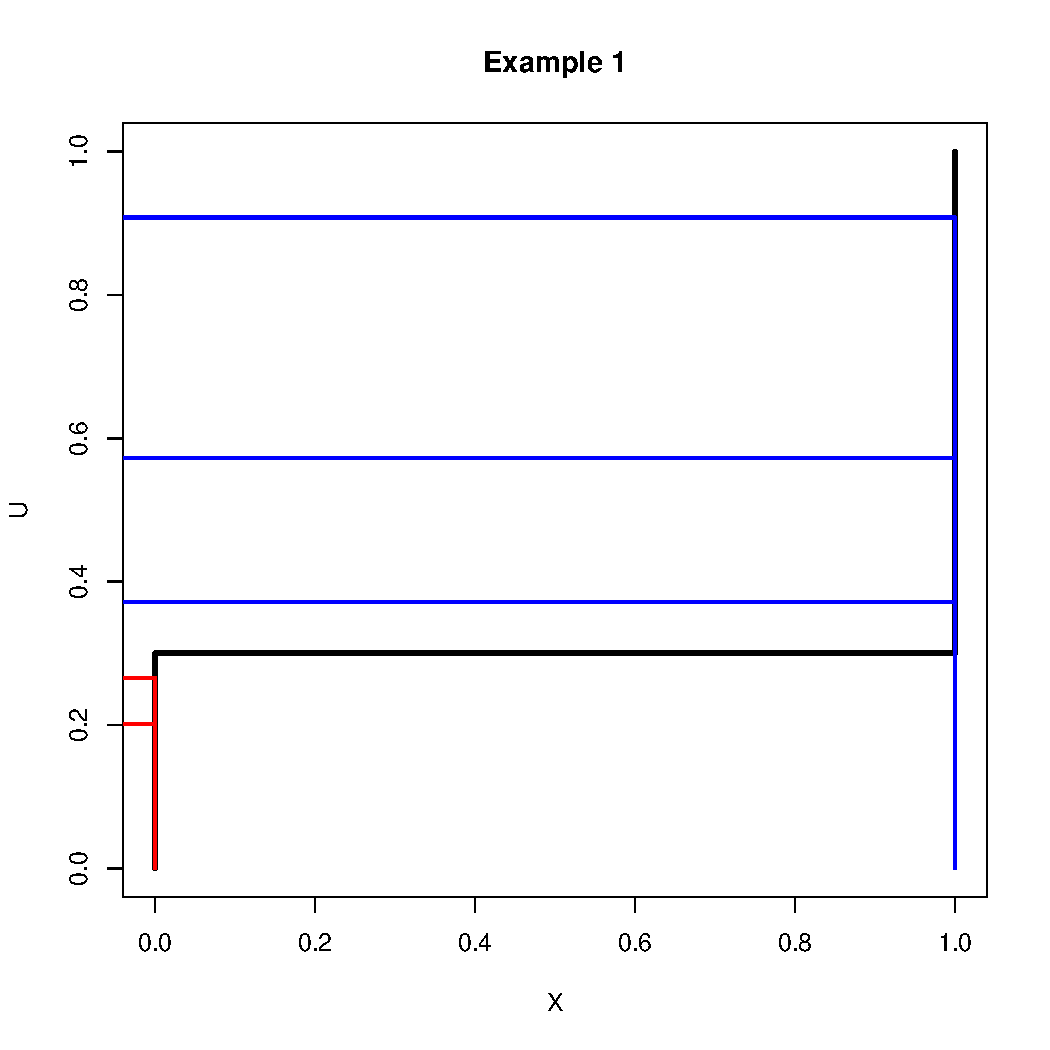
\includegraphics[height=7cm]{./Pics/d1p3.pdf}
\end{center}
\end{frame}
\begin{frame}{Visualization: Example 2}
\begin{center}
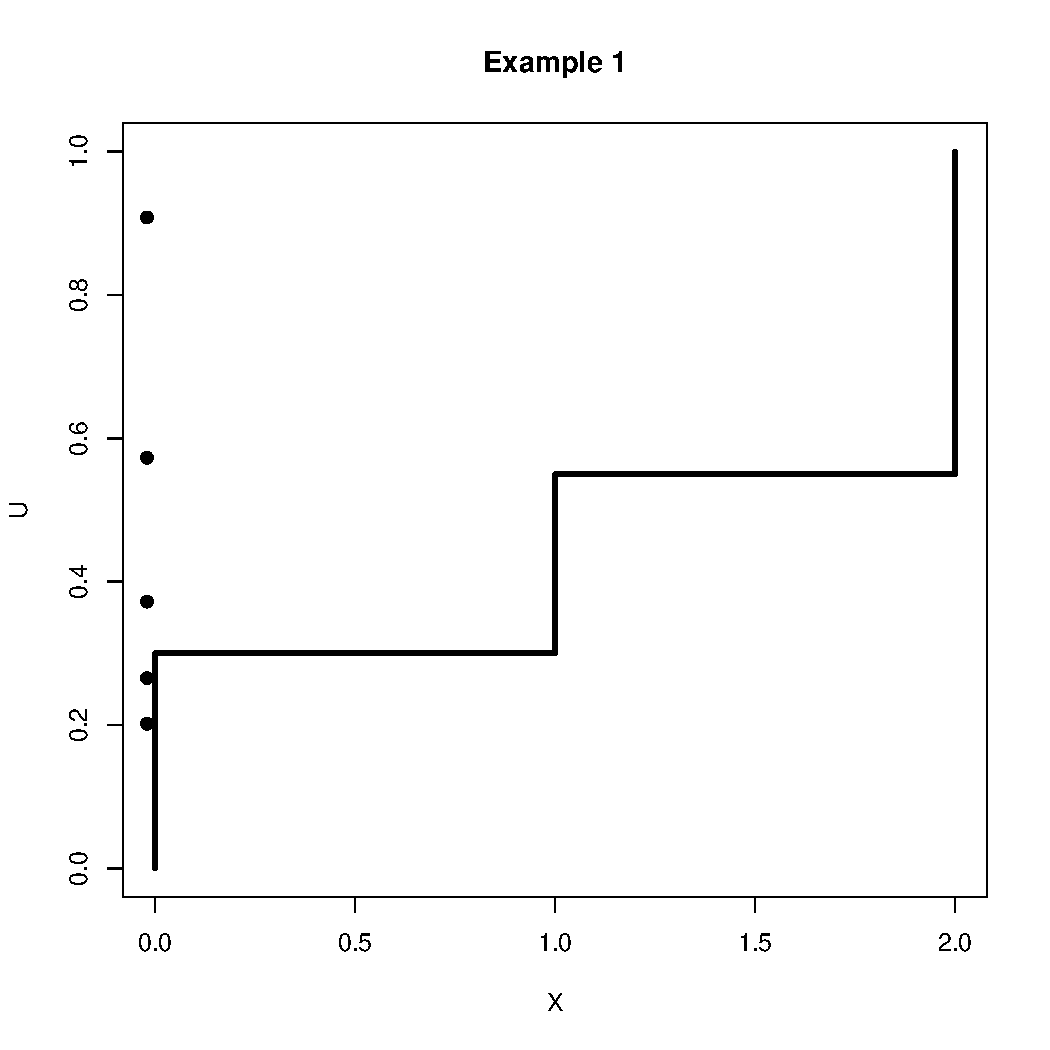
\includegraphics[height=7cm]{./Pics/d2p1.pdf}
\end{center}
\end{frame}
\begin{frame}{Visualization: Example 2}
\begin{center}
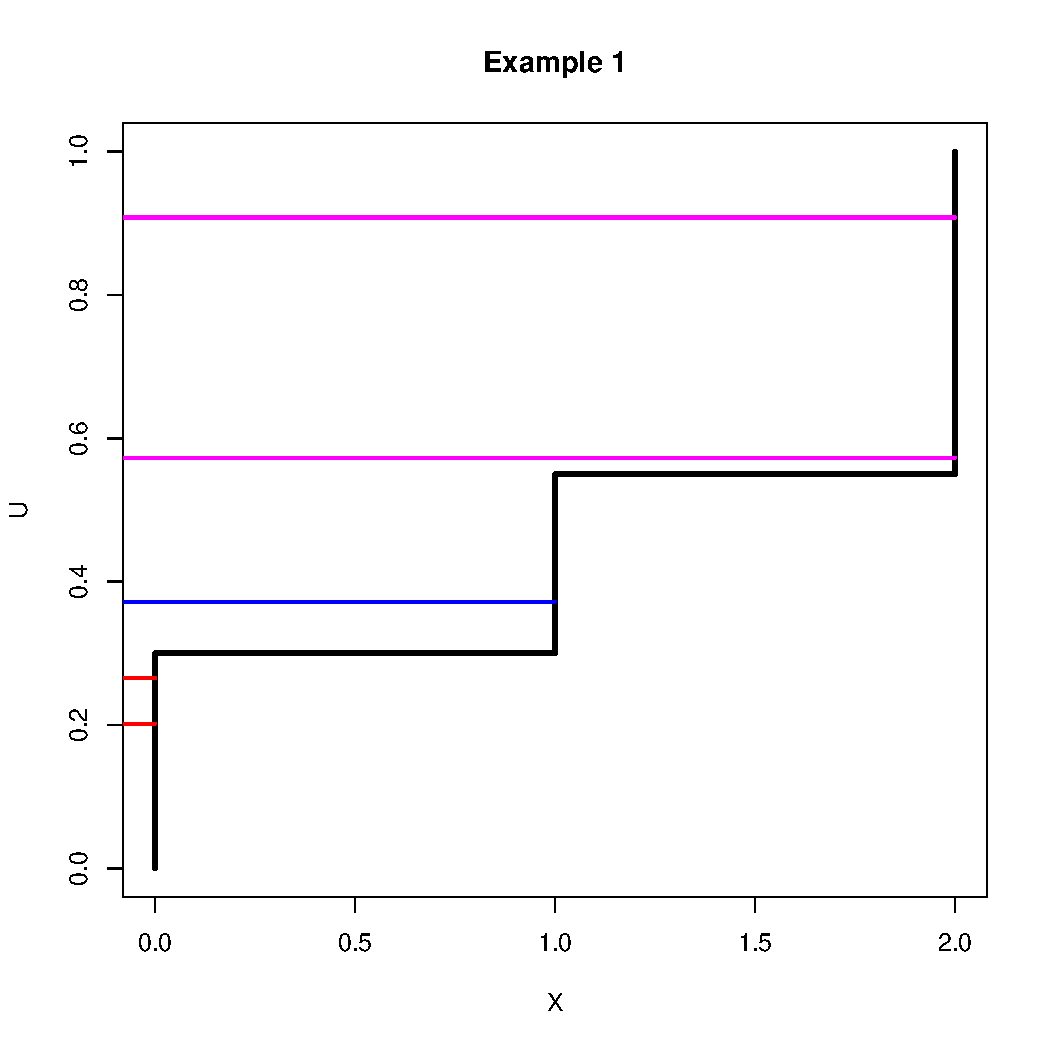
\includegraphics[height=7cm]{./Pics/d2p2.pdf}
\end{center}
\end{frame}
\begin{frame}{Visualization: Example 2}
\begin{center}
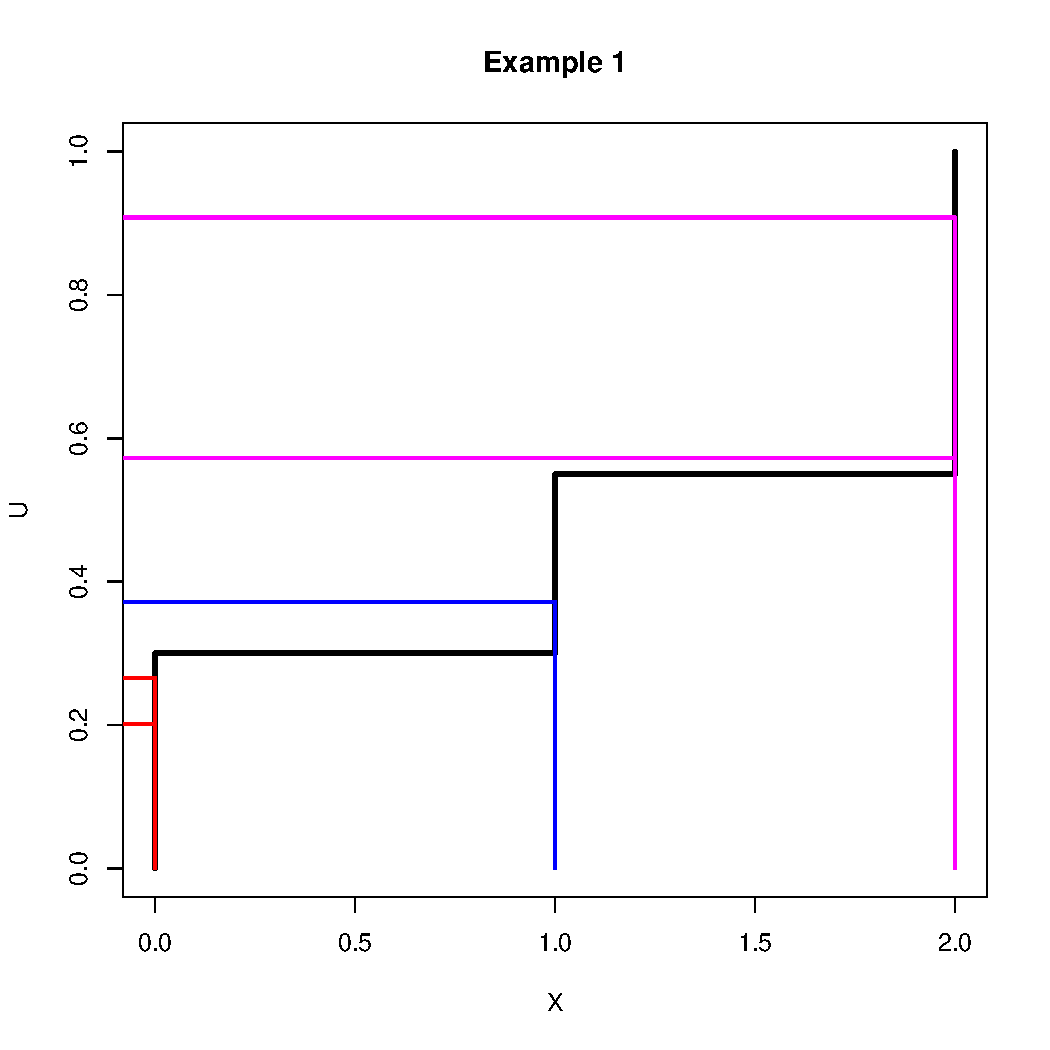
\includegraphics[height=7cm]{./Pics/d2p3.pdf}
\end{center}
\end{frame}
\subsection{Continuous Case}
\begin{frame}{Continuous Case}
\begin{itemize}
\item How do we extend this idea to the continuous case?
\pause
\item What was the step function in our discrete example?
\pause
\item It is the {\bf cumulative distribution function (cdf)}
\pause
\item Can we replace the discrete cdf with a continuous cdf?
\pause
\item Yes!
\end{itemize}
\end{frame}

\begin{frame}{Visualization: Continuous}
\begin{center}
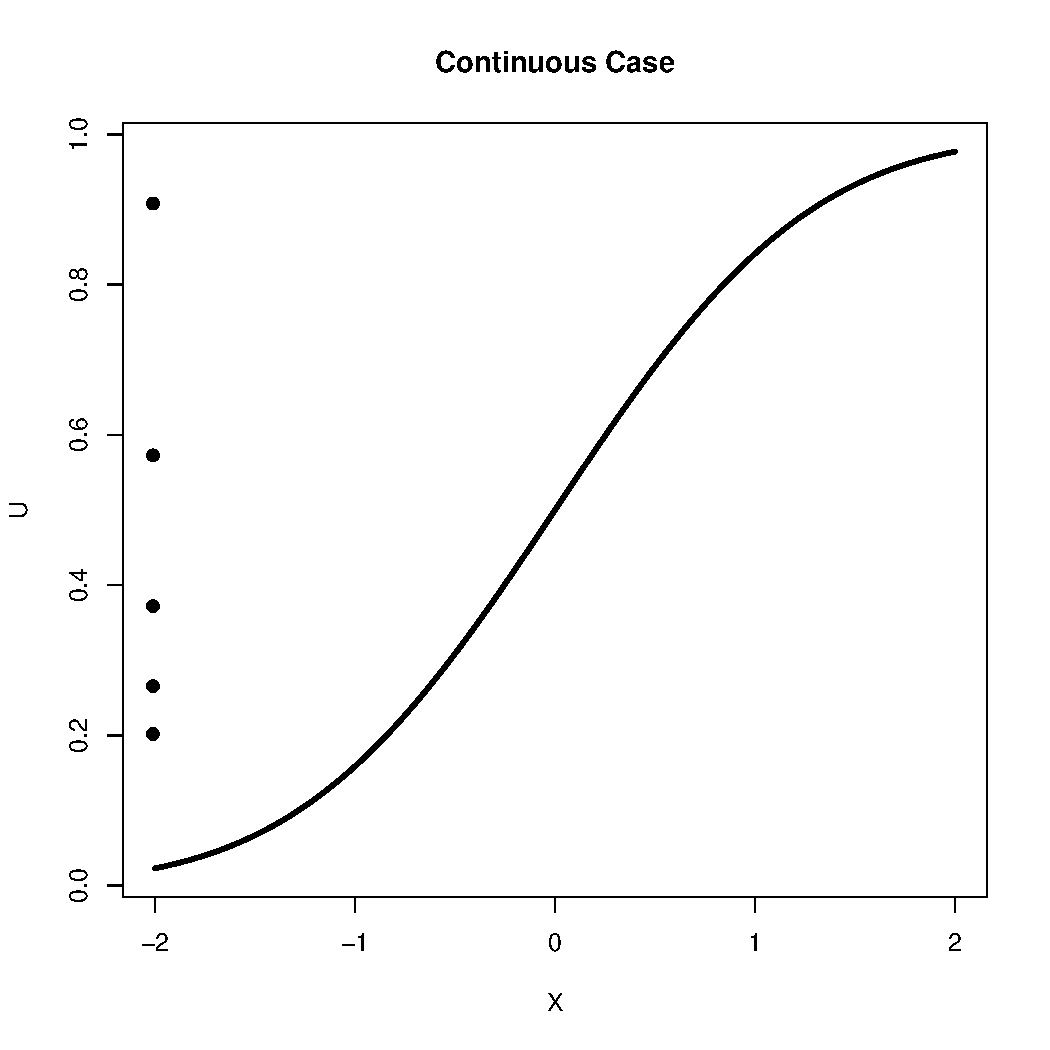
\includegraphics[height=7cm]{./Pics/cp1.pdf}
\end{center}
\end{frame}
\begin{frame}{Visualization: Continuous}
\begin{center}
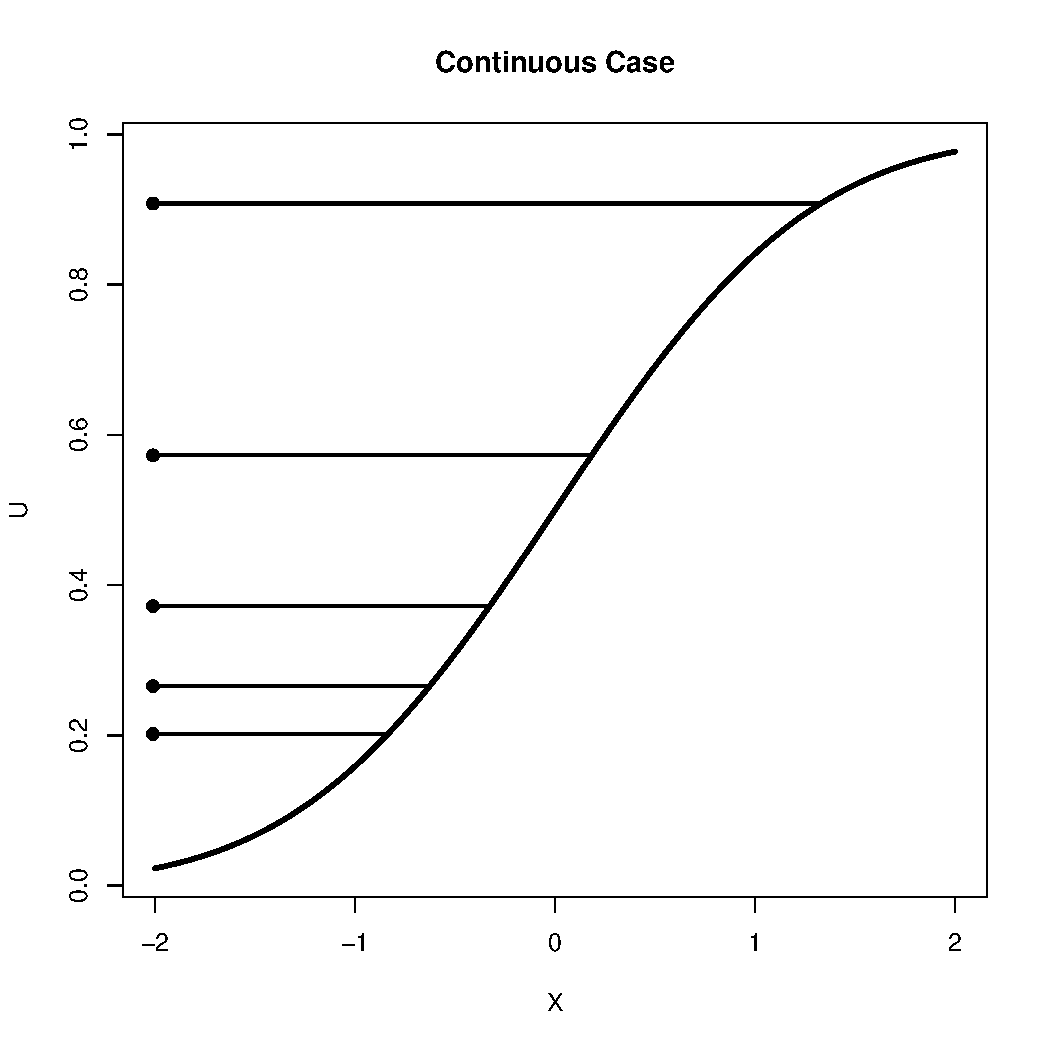
\includegraphics[height=7cm]{./Pics/cp2.pdf}
\end{center}
\end{frame}
\begin{frame}{Visualization: Continuous}
\begin{center}
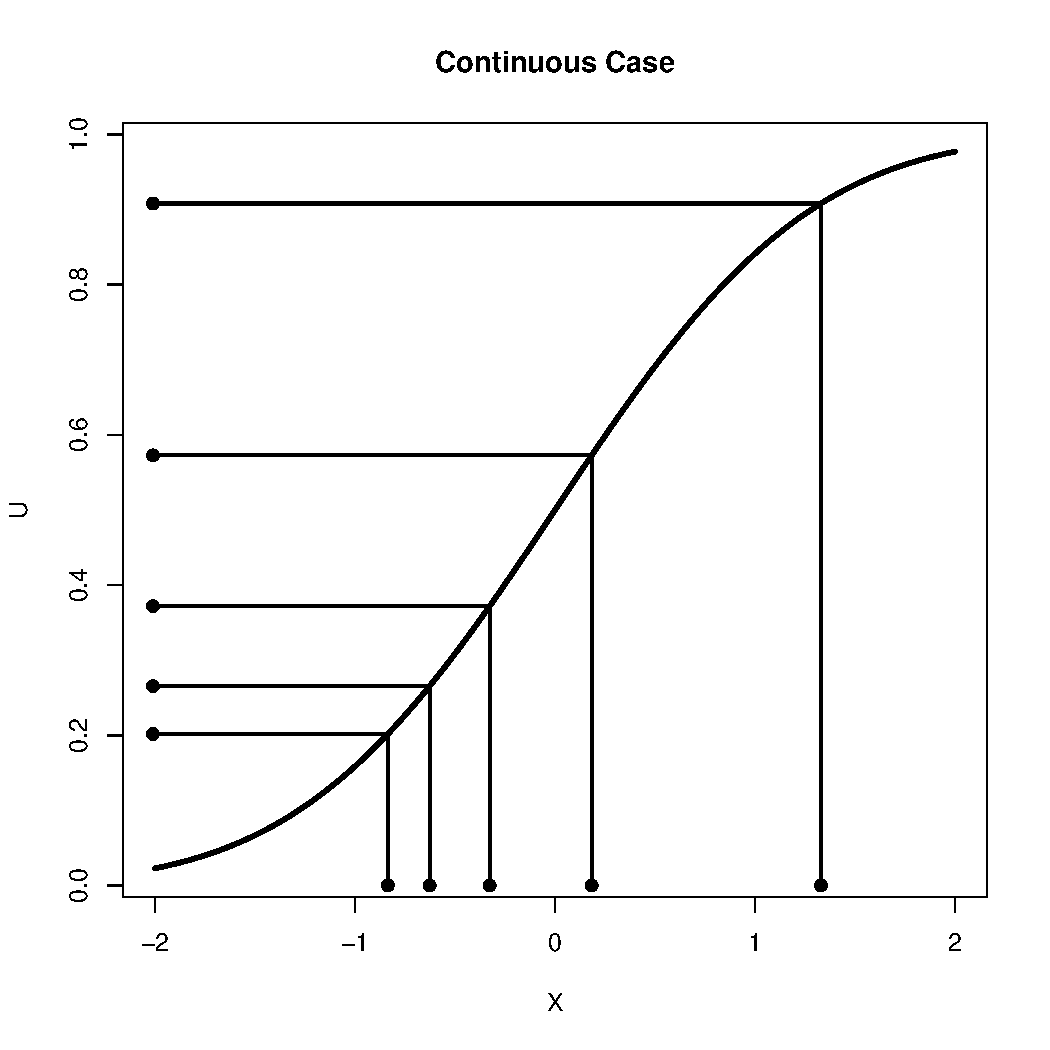
\includegraphics[height=7cm]{./Pics/cp3.pdf}
\end{center}
\end{frame}
\begin{frame}{Continuous Case}
\begin{itemize}
\item The cdf, $F(X)$ takes values of $X$ and gives a value between $0$ and $1$
\pause
\item Here we take values between $0$ and $1$ and get a value of $X$
\pause
\item What function do we use?
\pause
\item We use the {\bf Inverse cdf}
\end{itemize}
\end{frame}
\begin{frame}{The Direct Method}
\begin{itemize}
\item Two Steps:
\pause
\begin{enumerate}
\item Simulate $u\sim U(0,1)$
\item Set $x=F^{-1}(u)$
\end{enumerate}
\pause
\item This is why the {\bf direct method} is also called {\bf the inversion method}
\pause
\item Note that $F^{-1}(u)\neq\frac{1}{F(u)}$
\end{itemize}
\end{frame}
\begin{frame}{Your task}
\begin{itemize}
\item The CDF for an exponential distribution is
\begin{equation}
F(x)=1-e^{-\lambda x}
\end{equation}
\pause
\item Work out the inverse CDF
\pause
\item Simulate 1000 draws from the exponential distribution with $\lambda=1$ using the direct method.
\end{itemize}
\end{frame}
\begin{frame}{Your task}
\begin{itemize}
\item There are three ways to do it:
\pause
\begin{enumerate}
\item Write your own function to invert the CDF.
\item Use the R function {\em qexp} to invert the CDF.
\item Use the R function {\em rexp} to do everything.
\end{enumerate}
\pause
\item Do all three and compare:
\pause
\begin{itemize}
\item Histograms
\item Summary statistics (using R function {\em summary})
\end{itemize} 
\end{itemize}
\end{frame}
\begin{frame}{Functions in R}
\begin{itemize}
\item It is easy to simulate random distributions in R using {\em r*}, for example {\em rnorm}, {\em rbeta}, {\em rgamma}, {\em rchisq}, etc.
\pause
\item The inverse cdfs are given by {\em q*}, for example {\em qnorm}, {\em qbeta}, {\em qgamma}, {\em qchisq}, etc.
\pause
\item The cdfs are given by {\em p*}, for example {\em pnorm}, {\em pbeta}, {\em pgamma}, {\em pchisq}, etc.
\pause
\item The pdfs (densities) are given by {\em d*}, for example {\em dnorm}, {\em dbeta}, {\em dgamma}, {\em dchisq}, etc.
\end{itemize}
\end{frame}
\section{Indirect Simulation: Accept-Reject}
\begin{frame}{Indirect simulation}
\begin{itemize}
\item What if the cumulative distribution function is difficult to invert, or not even available?
\pause
\item How to invert the cdf of a standard normal distribution?
\pause
\begin{equation}
F(x)=\int_{-\infty}^{x}(2\pi)^{-1/2}e^{-x^2/2}dx
\end{equation}
\pause
\item It is still possible to simulate from this distribution?
\pause
\item If the {\bf density} is available, then the answer is YES!
\end{itemize}
\end{frame}
%\begin{frame}{Shooting arrows}
%\pause
%\begin{center}
%
\includegraphics[height=7cm]{./Pics/Li.jpeg}
%\end{center}
%\end{frame}
\begin{frame}{Approximating $\pi$}
\begin{center}
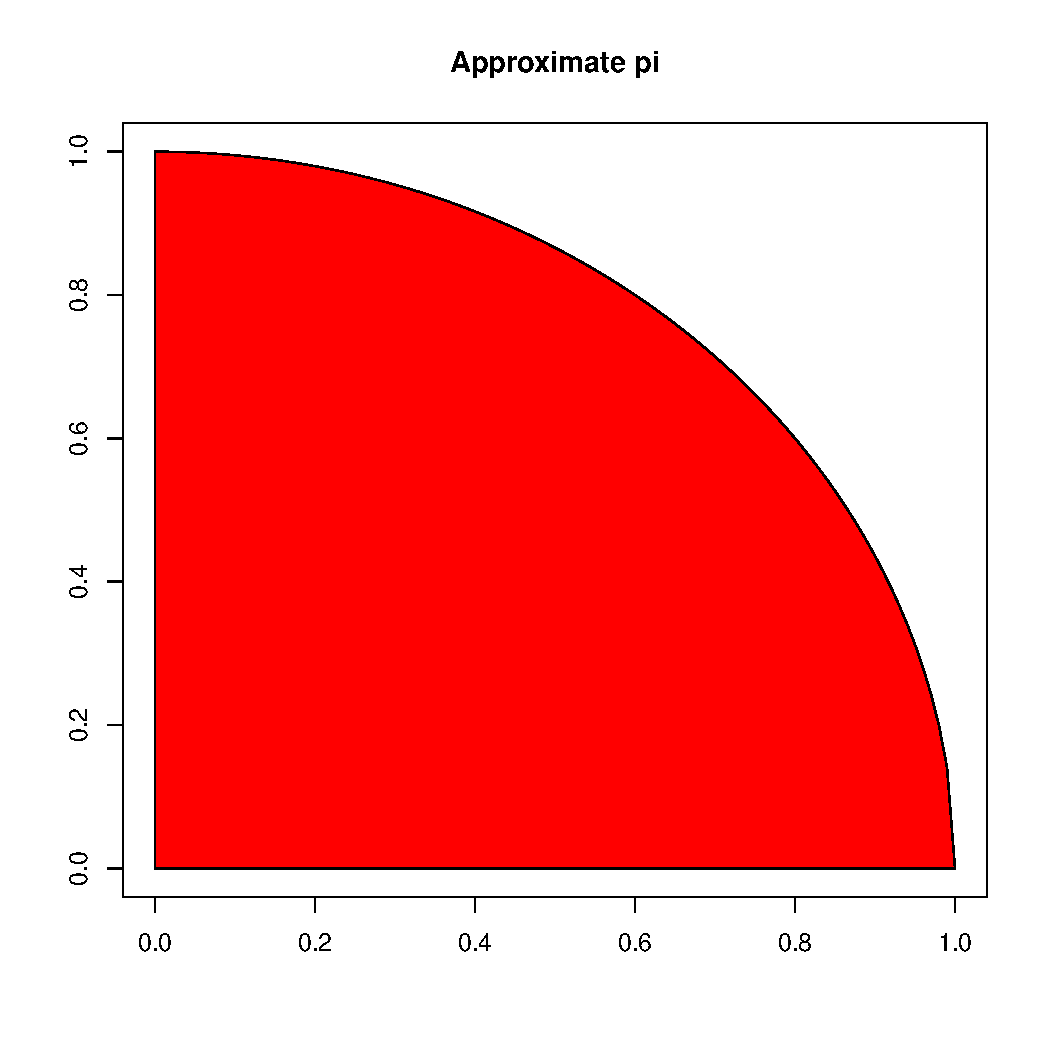
\includegraphics[height=7cm]{./Pics/appi1.pdf}
\end{center}
\end{frame}
\begin{frame}{Approximating $\pi$}
\begin{itemize}
\item The previous slide shows a quarter circle with radius 1
\pause
\item A full circle has area $\pi$ so the red area is $\pi/4\approx 0.7853982$.
\pause
\item Can we approximate $\pi$ by ``shooting arrows'' at the quarter circle. 
\end{itemize}
\end{frame}
\begin{frame}{Approximating $\pi$}
\begin{center}
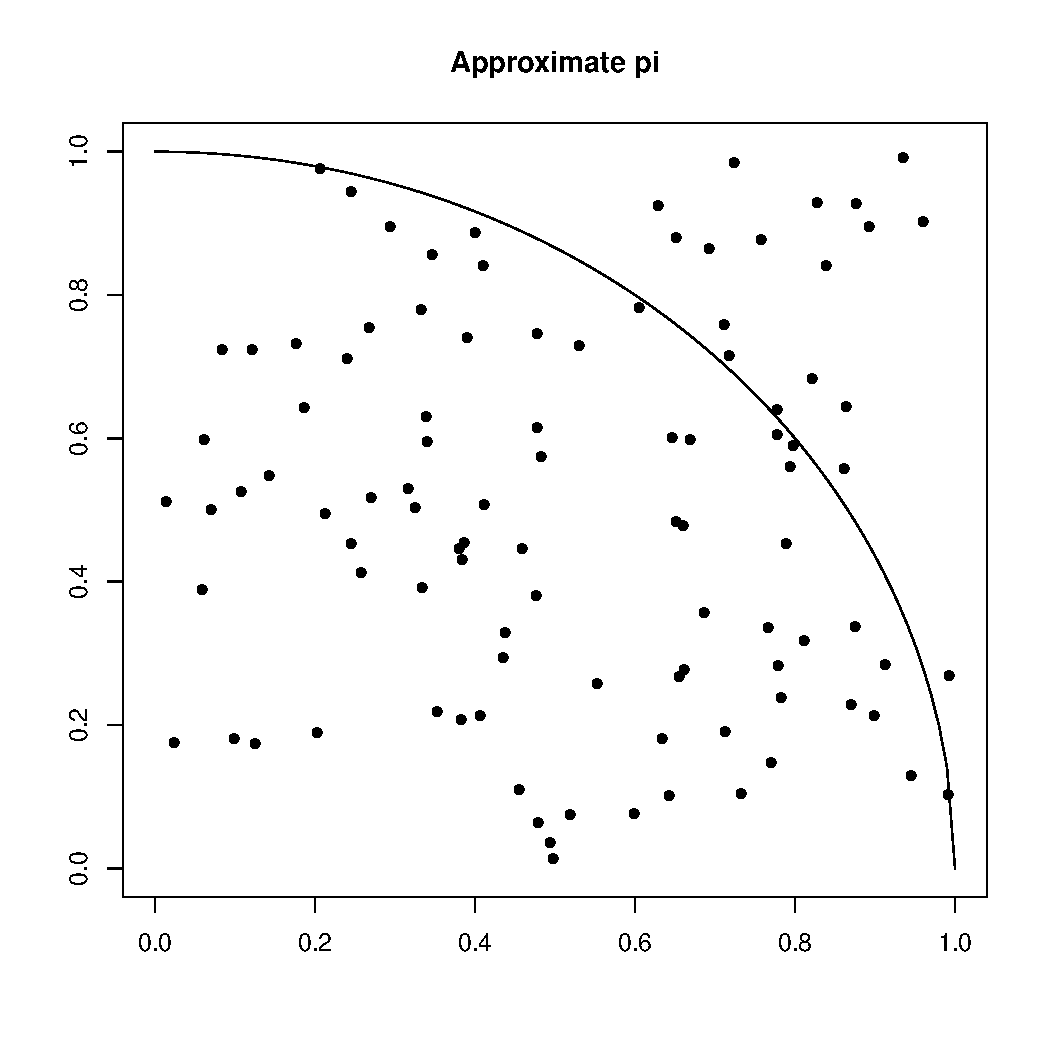
\includegraphics[height=7cm]{./Pics/appi2.pdf}
\end{center}
\end{frame}
\begin{frame}{Approximating $\pi$}
\begin{center}
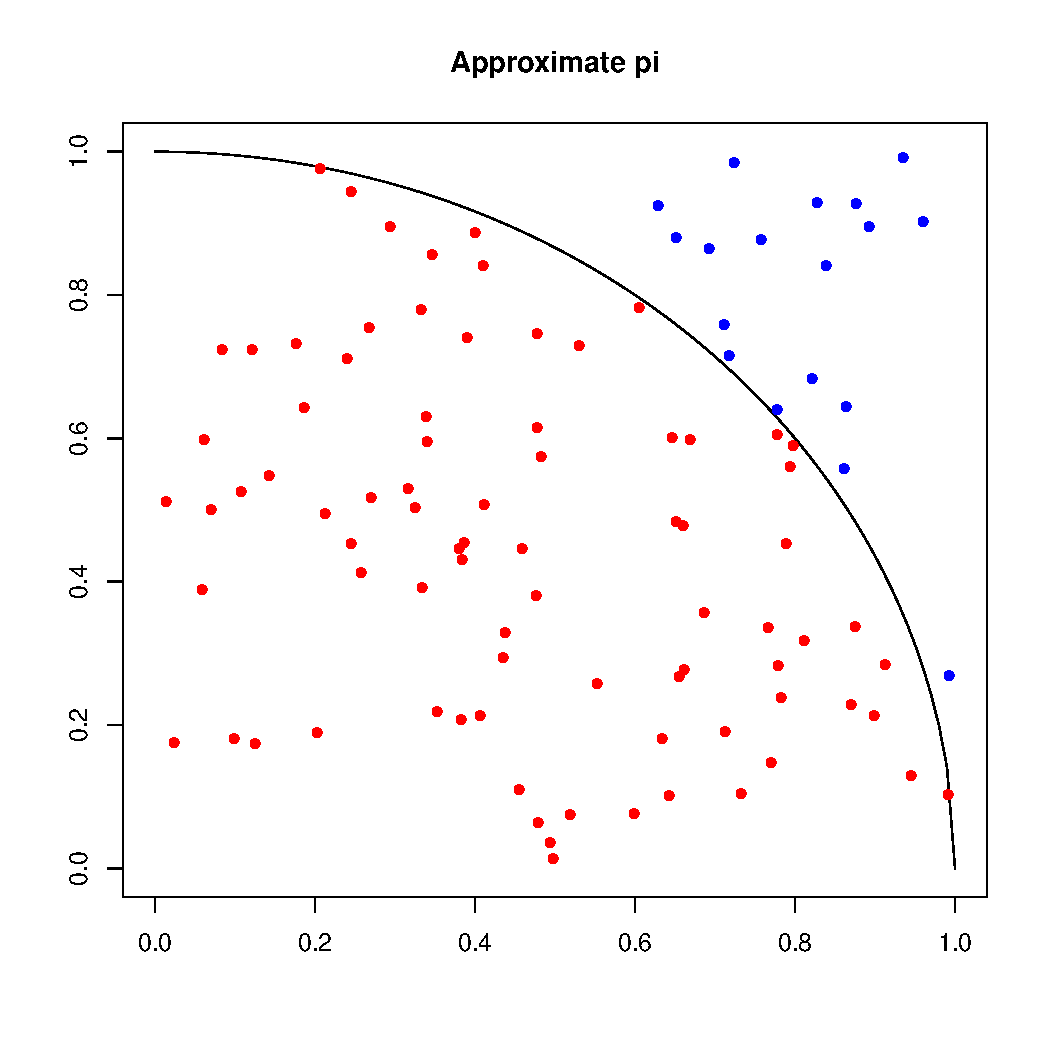
\includegraphics[height=7cm]{./Pics/appi3.pdf}
\end{center}
\end{frame}
\begin{frame}{Approximating $\pi$}
An approximation for $\pi/4$ is
\pause
\begin{equation*}
\pi/4\approx\frac{\mbox{Number of Red Points}}{\mbox{Number of Red Points}+\mbox{Number of Blue Points}}
\end{equation*}
Try this

\end{frame}
\begin{frame}{Monte Carlo methods}
\begin{itemize}
\item Notice that this exercise is the same as evaluating the integral
\begin{equation}
\int_0^1 \sqrt{(1-x^2)}dx
\end{equation}
\pause
\item Methods that use simulation to estimate integrals are known as {\bf Monte Carlo} methods.
\end{itemize}
\end{frame}
\begin{frame}{`Shooting' a density}
\begin{itemize}
\item We now `shoot arrows' at a density function 
\pause
\item Consider the Beta distribution: 
\begin{equation}
\mbox{Beta}(z;a,b)=\frac{\Gamma(a+b)}{(\Gamma(a)\Gamma(b))}z^{a-1}(1-z)^{b-1}
\end{equation}
\pause
\item Let $a=b=2$ 
\end{itemize}
\end{frame}
\begin{frame}{Beta density}
\begin{center}
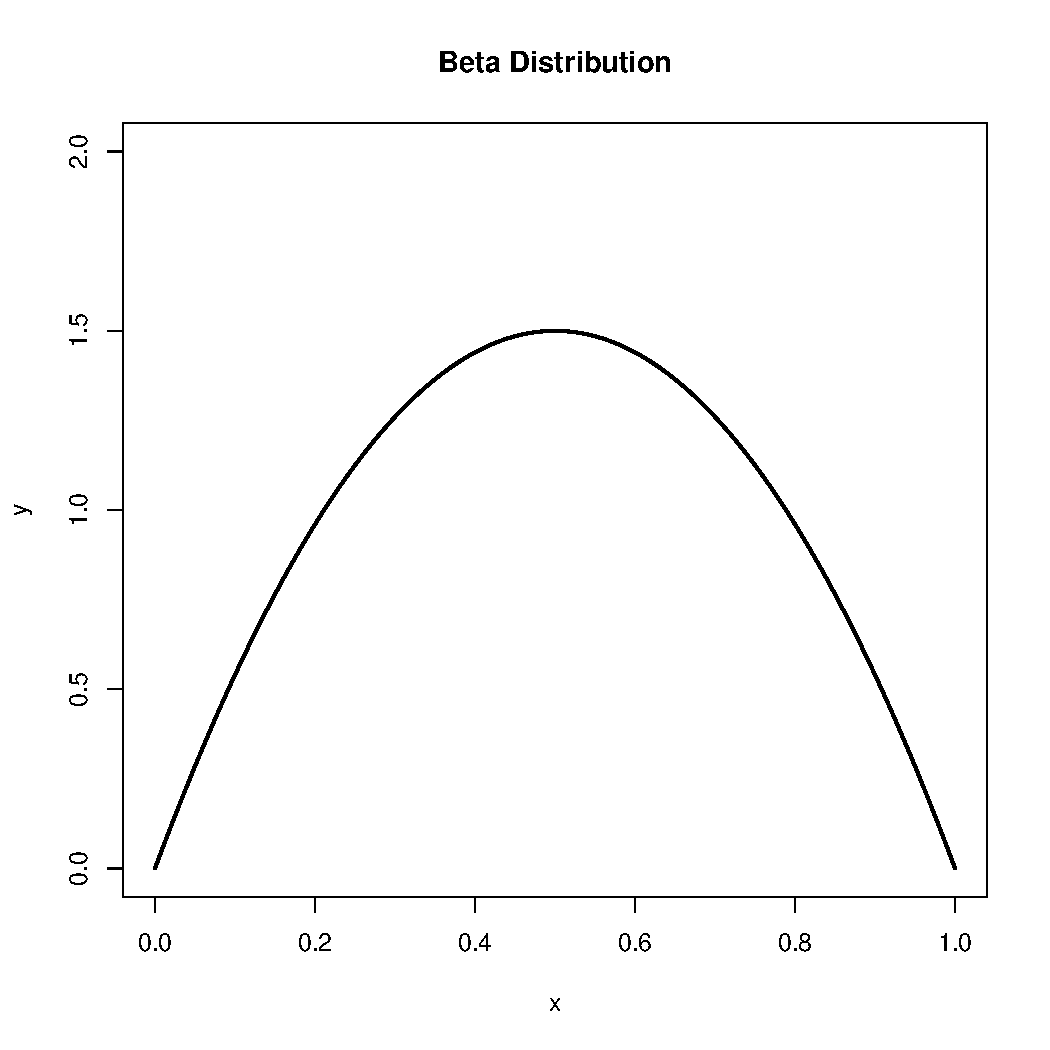
\includegraphics[height=7cm]{./Pics/bet1.pdf}
\end{center}
\end{frame}
\begin{frame}{Beta density}
\begin{itemize}
\item Note that we cannot just shoot arrows in $[0,1]^2$
\pause
\item The domain of the Beta density function is $\left[0,1\right]$ so the x coordinates can be from U(0,1)
\pause
\item The range of the Beta density function with $a=b=2$ is wider than $\left[0,1\right]$.
\pause
\item Instead let the y coordinates of the `arrows' must lie in $\left[0,M\right]$
\pause
\item The y coordinates can be simulated from $U(0,1)$ and multiplied by $M$.
\pause
\item For now, let $M=2$
\end{itemize}
\end{frame}
\begin{frame}{Beta density}
\begin{center}
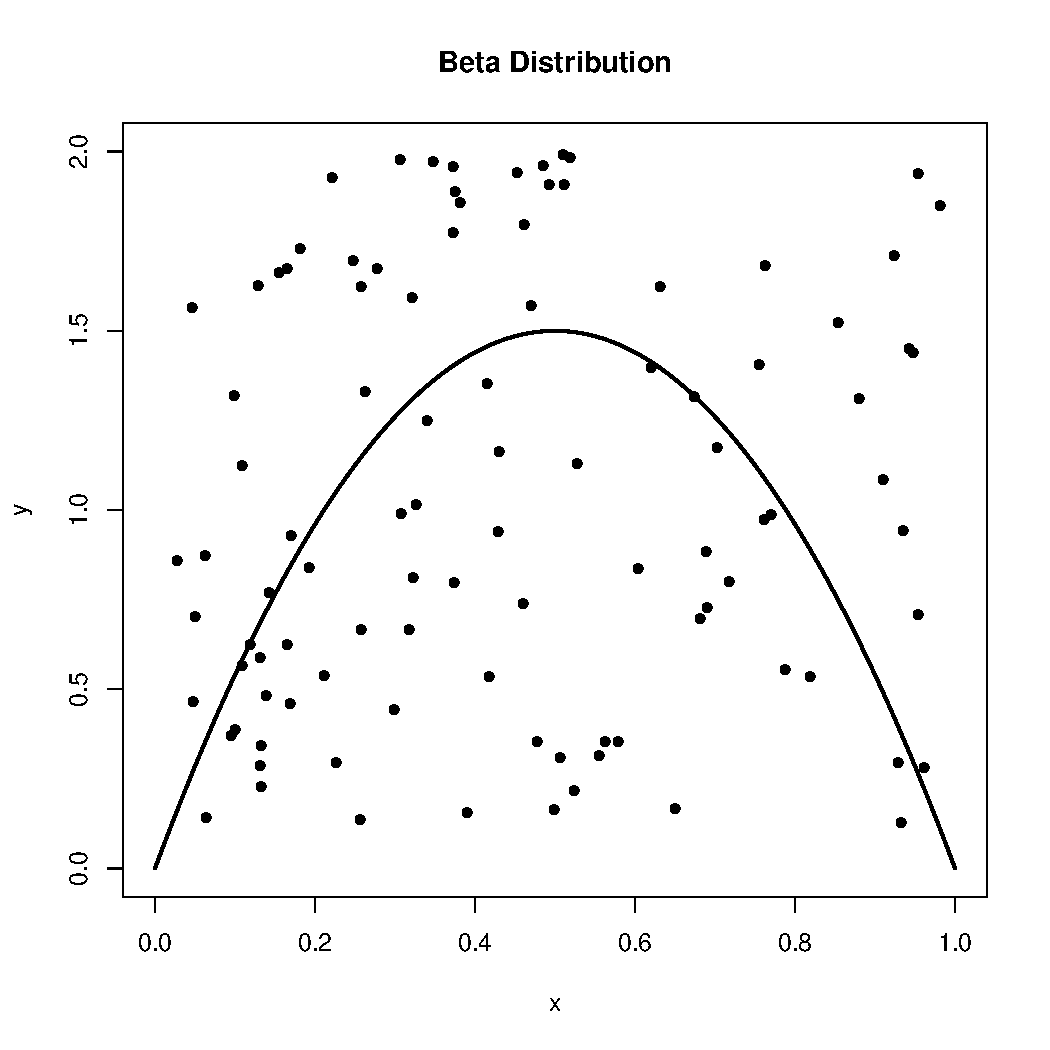
\includegraphics[height=7cm]{./Pics/bet2.pdf}
\end{center}
\end{frame}
\begin{frame}{Beta density}
\begin{center}
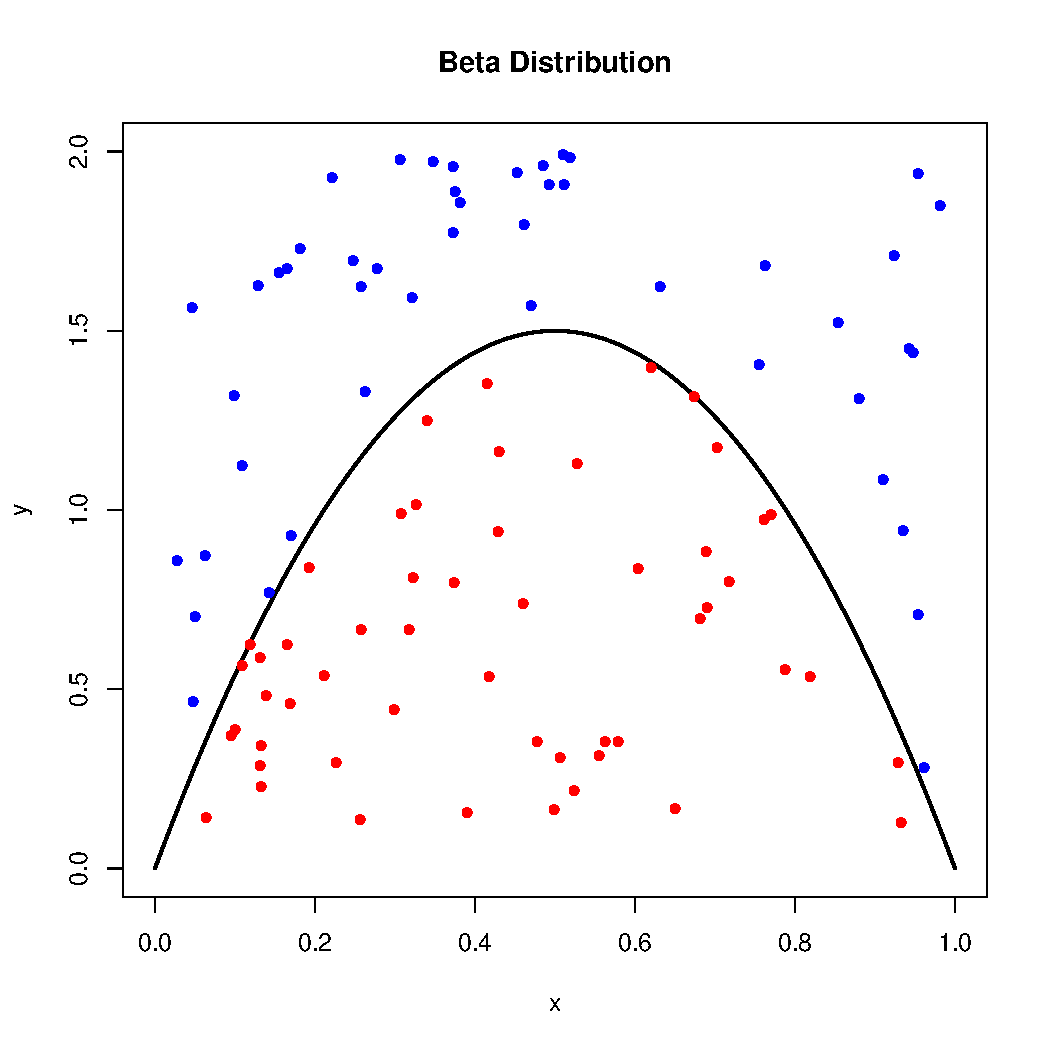
\includegraphics[height=7cm]{./Pics/bet3.pdf}
\end{center}
\end{frame}
\begin{frame}{Proportion of red arrows}
\begin{itemize}
\item What is the approximate proportion of red points to the total number of points?
\pause
\begin{equation*}
\frac{\mbox{No. of Red Points}}{\mbox{No. of Red points+No. of Blue Points}}
\end{equation*}
\pause
\item Hint: What is the area under the Beta density?
\end{itemize}
\end{frame}
\begin{frame}{Beta density}
\begin{center}
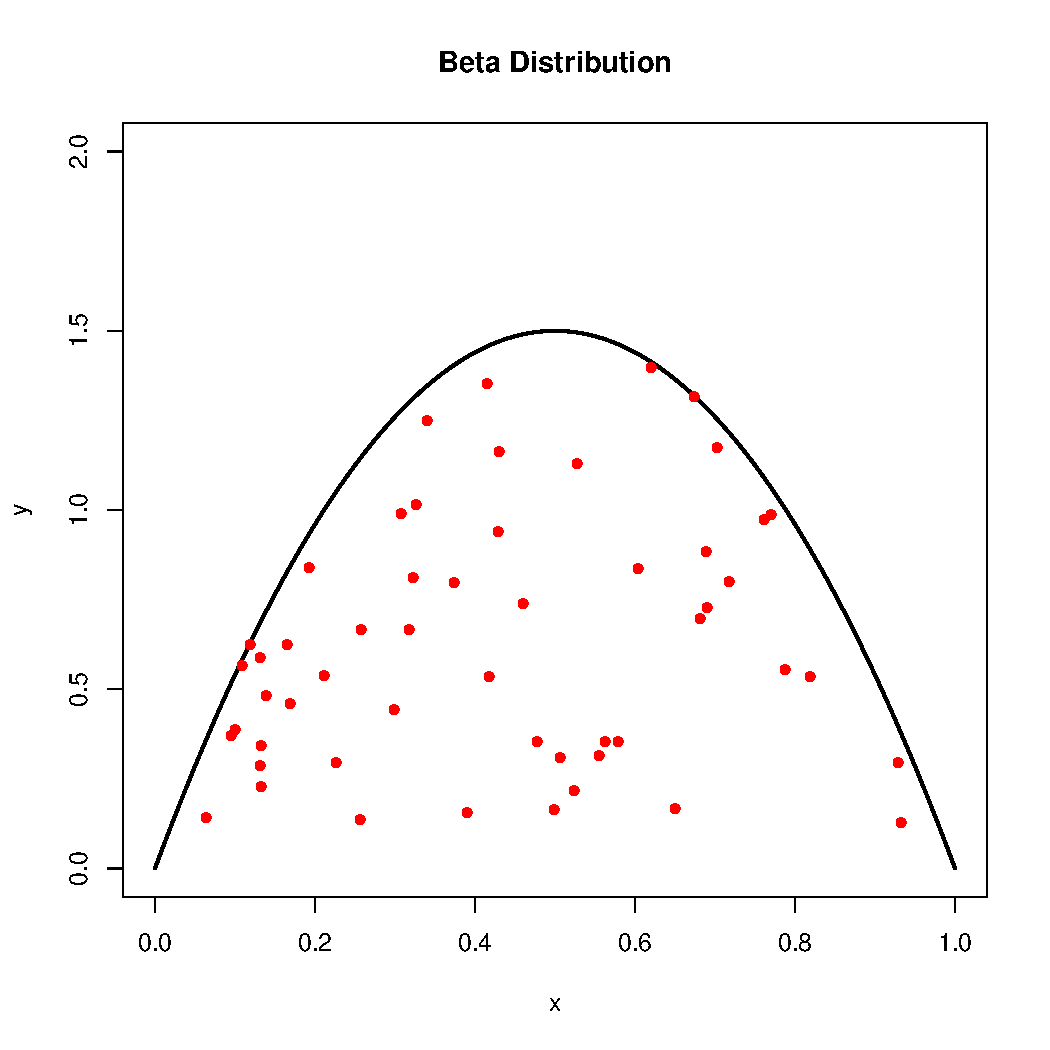
\includegraphics[height=7cm]{./Pics/bet4.pdf}
\end{center}
\end{frame}
\begin{frame}{Reject Blue Points}
\begin{itemize}
\item Suppose we only keep red points
\pause
\item Now consider the points which have an x coordinate greater than 0.5
\pause
\item Approximately what proportion of the dots will have $x>0.5$?
\pause
\item On the next diagram what is
\begin{equation}
\frac{\mbox{No. of Purple Points}}{\mbox{No. of Red points+No. of Purple Points}}
\end{equation}
\end{itemize}
\end{frame}
\begin{frame}{Beta density}
\begin{center}
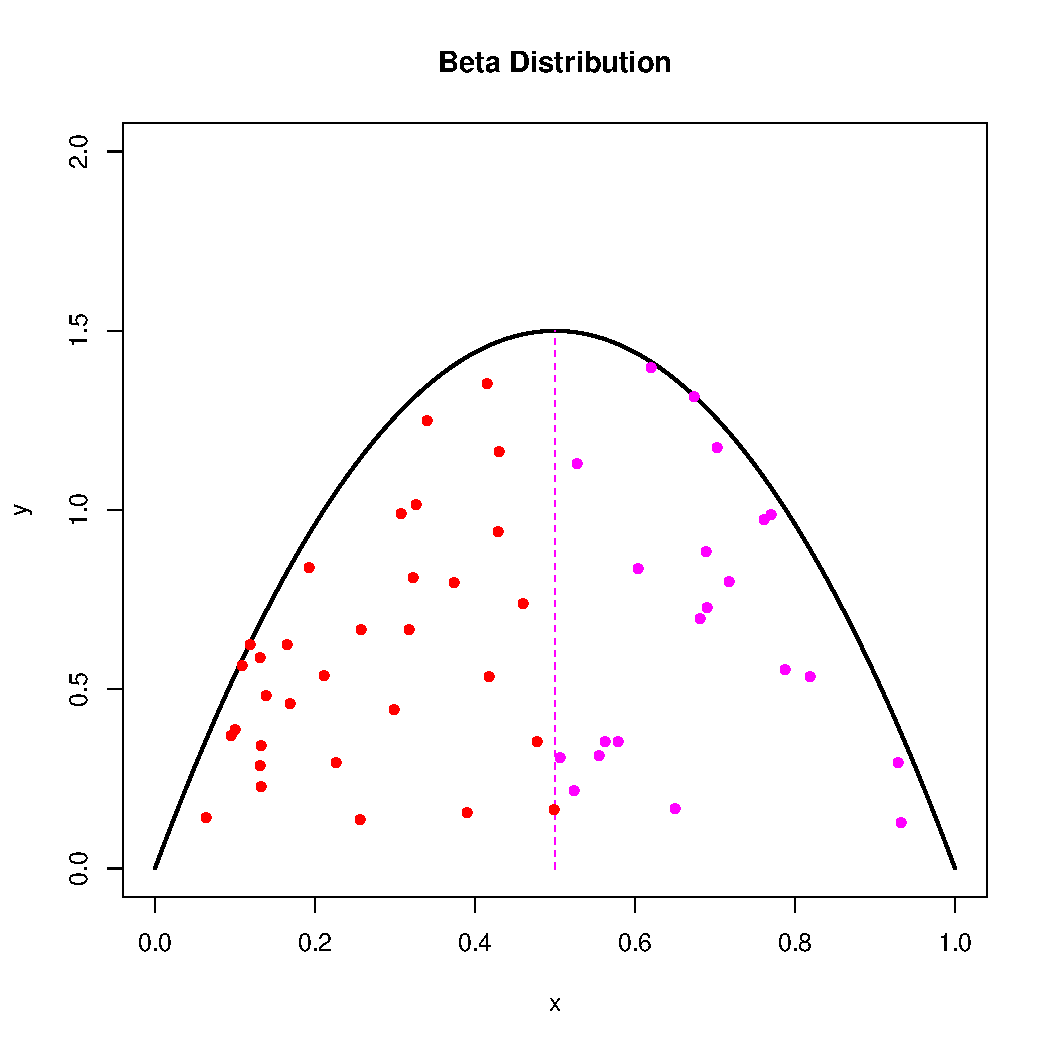
\includegraphics[height=7cm]{./Pics/bet5.pdf}
\end{center}
\end{frame}
\begin{frame}{Approximately 50\% of arrows are purple}
\begin{itemize}
\item What is the probability that $x>0.5$.\pause ~If
\pause
\begin{itemize}
\item We only consider arrows that fall inside the density function
\item If we only look at the x coordinate of those arrows
\end{itemize}
\pause
\item There is a 50\% probability that the x coordinate is greater than 0.5.
\pause
\item This is the same probability that a Beta(2,2) distributed variable is greater than 0.5. 
\pause
\item This works with any area under the density
\end{itemize}
\end{frame}

\begin{frame}{Approximately 20\% of arrows are purple}
\begin{center}
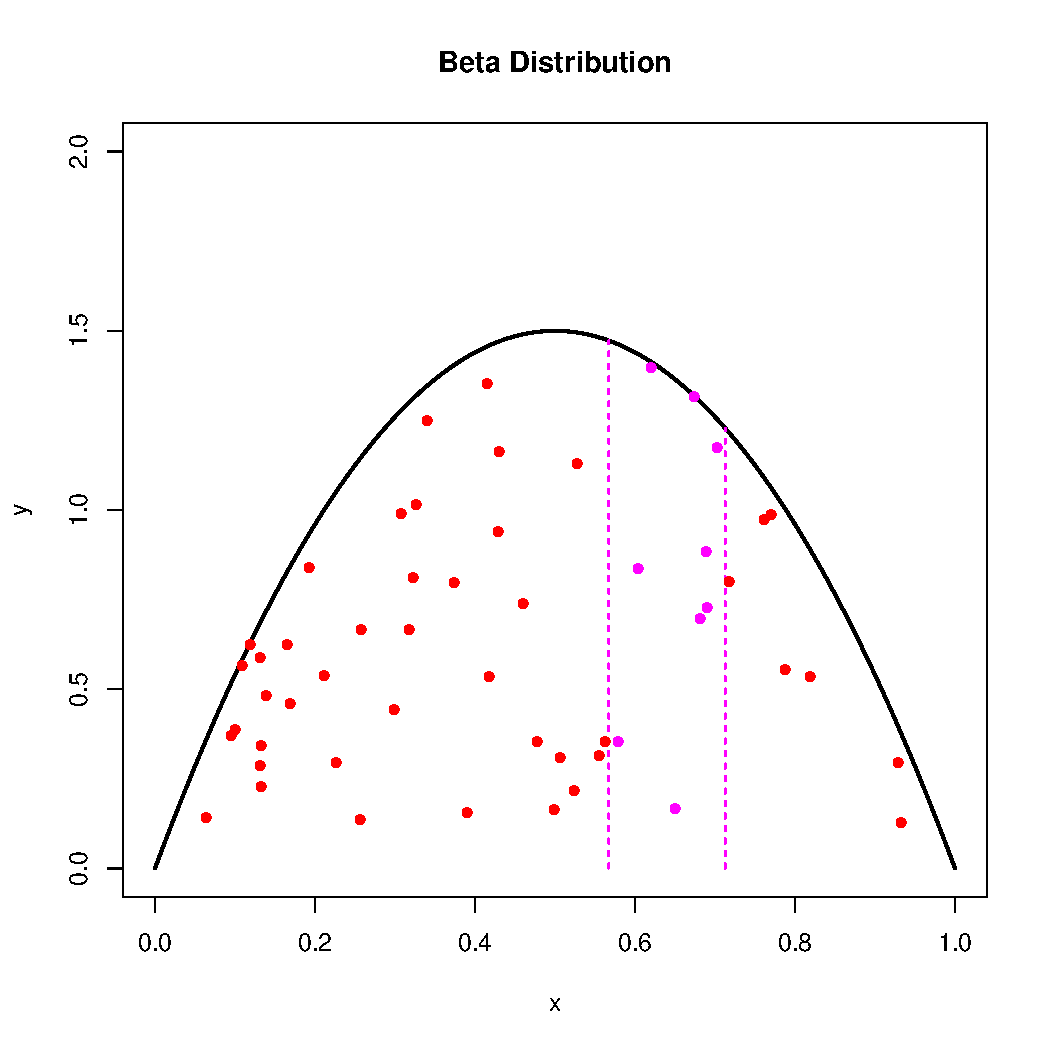
\includegraphics[height=7cm]{./Pics/bet6.pdf}
\end{center}
\end{frame}
\begin{frame}{Areas and Probabilities}
\begin{itemize}
\item What is an area under a density?
\pause
\item Mathematically, what is
\begin{equation*}
\int_a^b p(x)dx
\end{equation*}
\pause
\item It is a {\bf probability}
\begin{equation*}
\mbox{Pr}(a\leq x\leq b)=\int_a^b p(x)dx
\end{equation*}
\end{itemize}
\end{frame}
\begin{frame}{Writing this as an algorithm}
\begin{enumerate}
\item Generate $x\sim U(0,1)$
\item Generate $y\sim U(0,1)$
\item If \alt{$y<p(x)/M$}{$My<p(x)$}<2->, where $p(x)$ is the density of $\mbox{Beta}(2,2)$ 
\begin{itemize}
\item Keep $x$ 
\end{itemize}
Otherwise
\begin{itemize}
\item Reject $x$ 
\end{itemize}
\end{enumerate}
\pause\pause The $x$ that we keep follow a Beta (2,2) distribution.\\  \pause Now try to code this
\end{frame}
\begin{frame}{Can we do better?}
\begin{center}
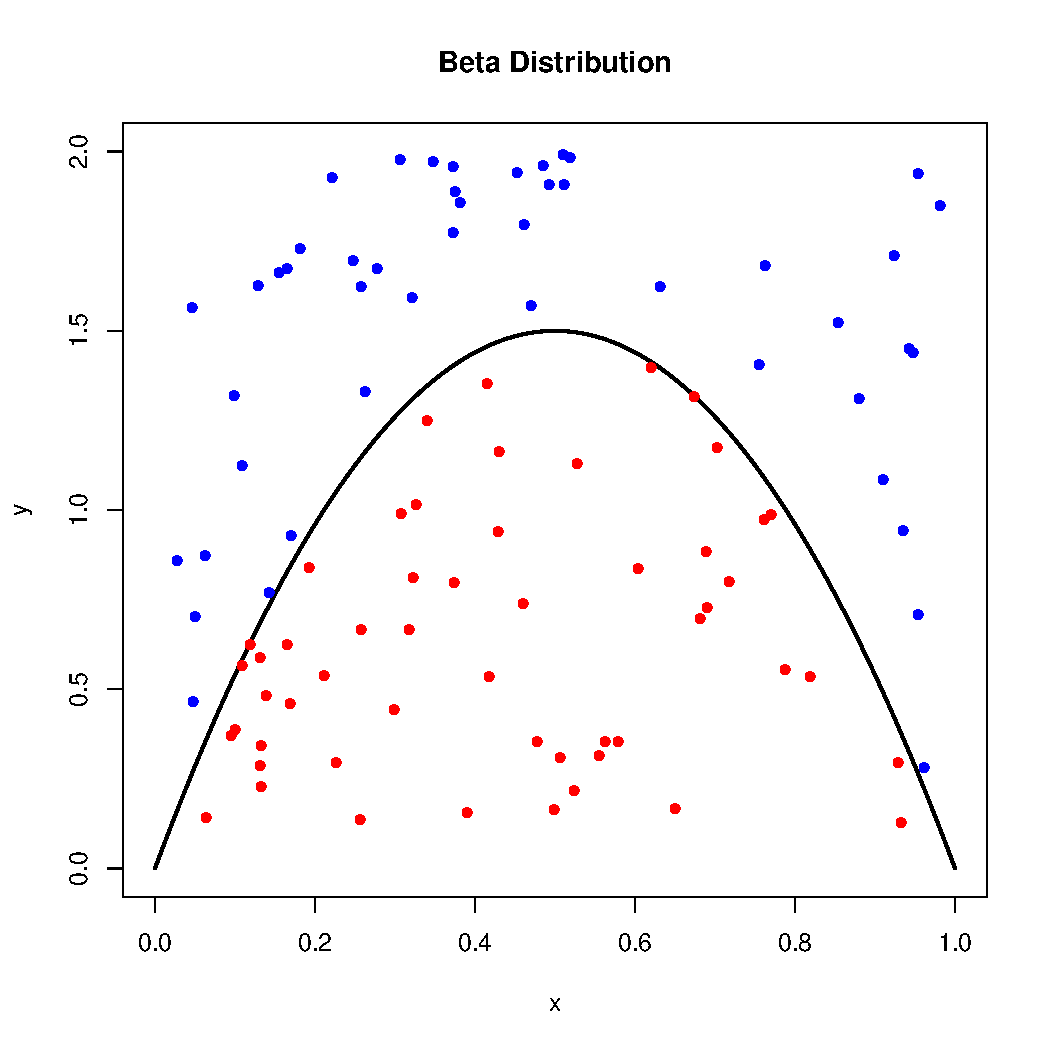
\includegraphics[height=7cm]{./Pics/bet3.pdf}
\end{center}
\end{frame}
\begin{frame}{Can we do better?}
\begin{itemize}
\item On the previous diagram many draws are wasted, especially in the region $y>1.5$.
\pause
\item The easiest way to improve this algorithm is to choose a better value of $M$.
\pause
\item The most efficient choice is
\begin{equation}
M=\sup_x p(x)
\end{equation}
\pause
\item For the Beta(2,2) distribution, the best choice is $M=1.5$.\\
\pause Try this. How many points do you reject?  How does it compare to when $M=2$
\end{itemize}
\end{frame}
\begin{frame}{Wasted points}
\begin{center}
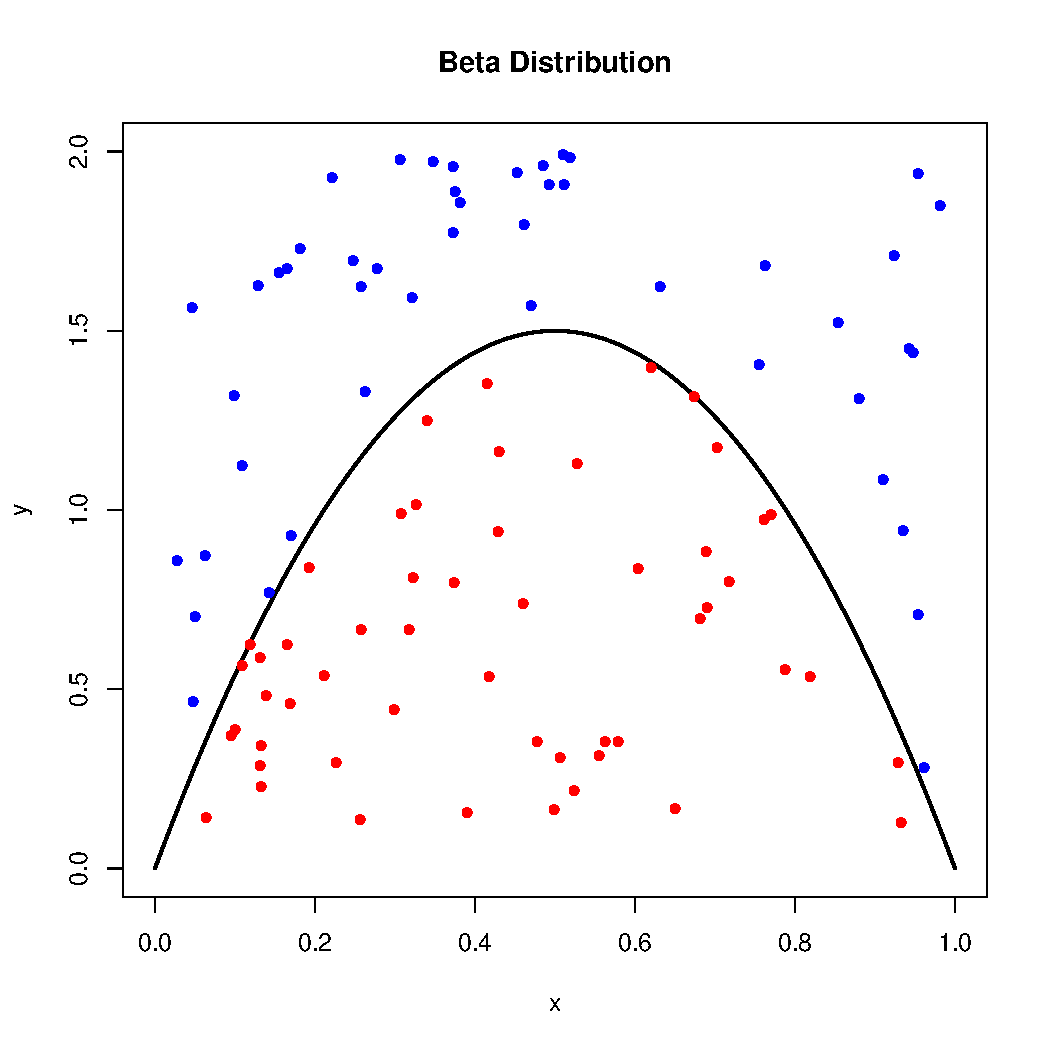
\includegraphics[height=7cm]{./Pics/bet3.pdf}
\end{center}
\end{frame}
\begin{frame}{Can we do even better?}
\begin{itemize}
\item We still waste a lot of iterates in the corners top left and top right corner of the previous plot.
\pause
\item Also how can we simulate from a distribution that has a domain from $-\infty$ to $\infty$? 
\pause
\item For example how can we adapt this algorithm to simulate from the normal distribution.
\pause
\item Over the next few slides we simulate from a normal distribution using the {\bf logistic} distribution as a {\bf proposal}
\end{itemize}
\end{frame}
\begin{frame}{Logistic distribution}
\begin{itemize}
\item The logistic distribution has distribution function
\begin{equation}
F(z)=(1+e^{-z})^{-1}
\end{equation}
\pause
\item The logistic distribution has density function
\begin{equation}
f(x)=\frac{e^z}{(1+e^z)^{2}}
\end{equation}
\pause
\item It is similar to the normal but has fatter tails.
\pause
\item It is easy to simulate from this distribution using the direct method.
\end{itemize}
\end{frame}
\begin{frame}{Normal v Logistic}
\begin{center}
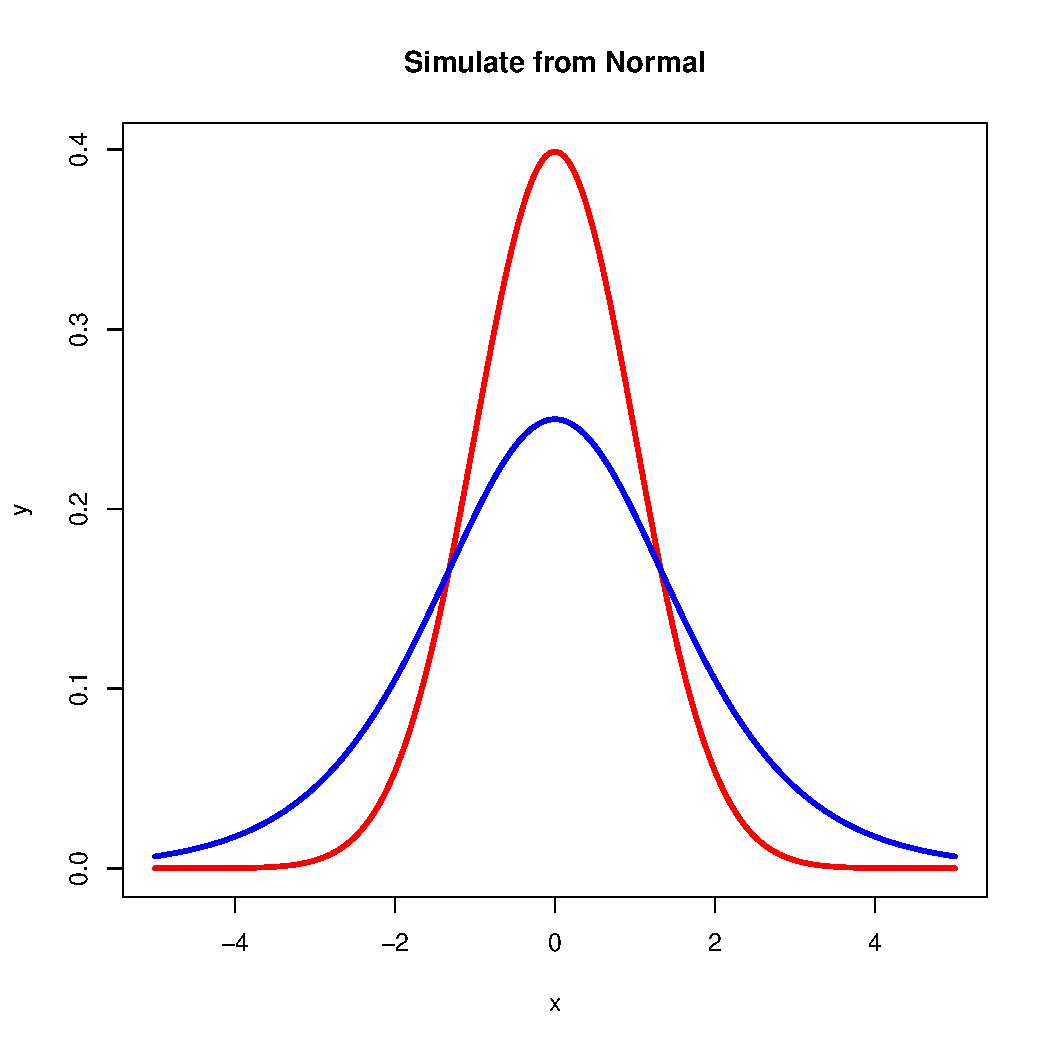
\includegraphics[height=7cm]{./Pics/nmlg1.pdf}
\end{center}
\end{frame}
\begin{frame}{Normal v Logistic}
\begin{center}
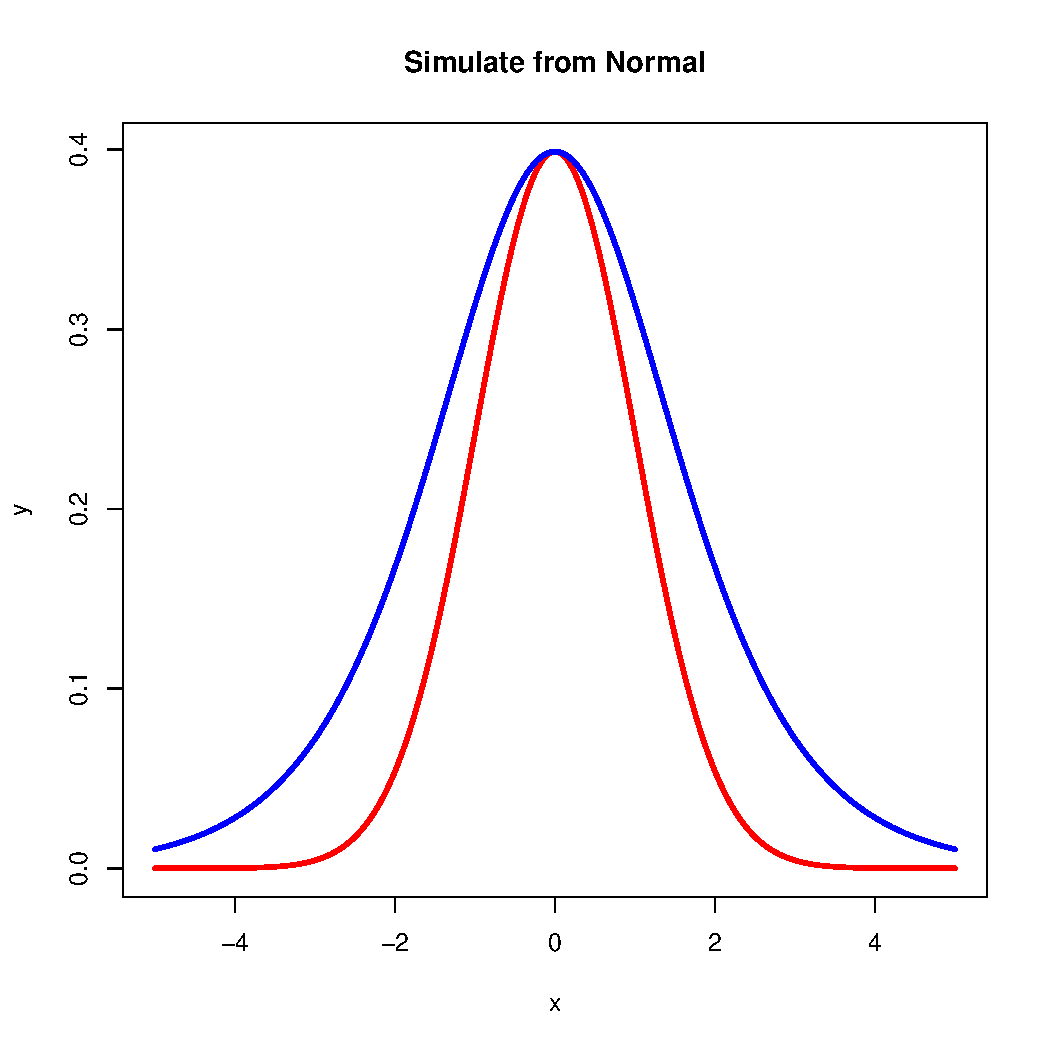
\includegraphics[height=7cm]{./Pics/nmlg2.pdf}
\end{center}
\end{frame}
\begin{frame}{Normal v Logistic}
\begin{center}
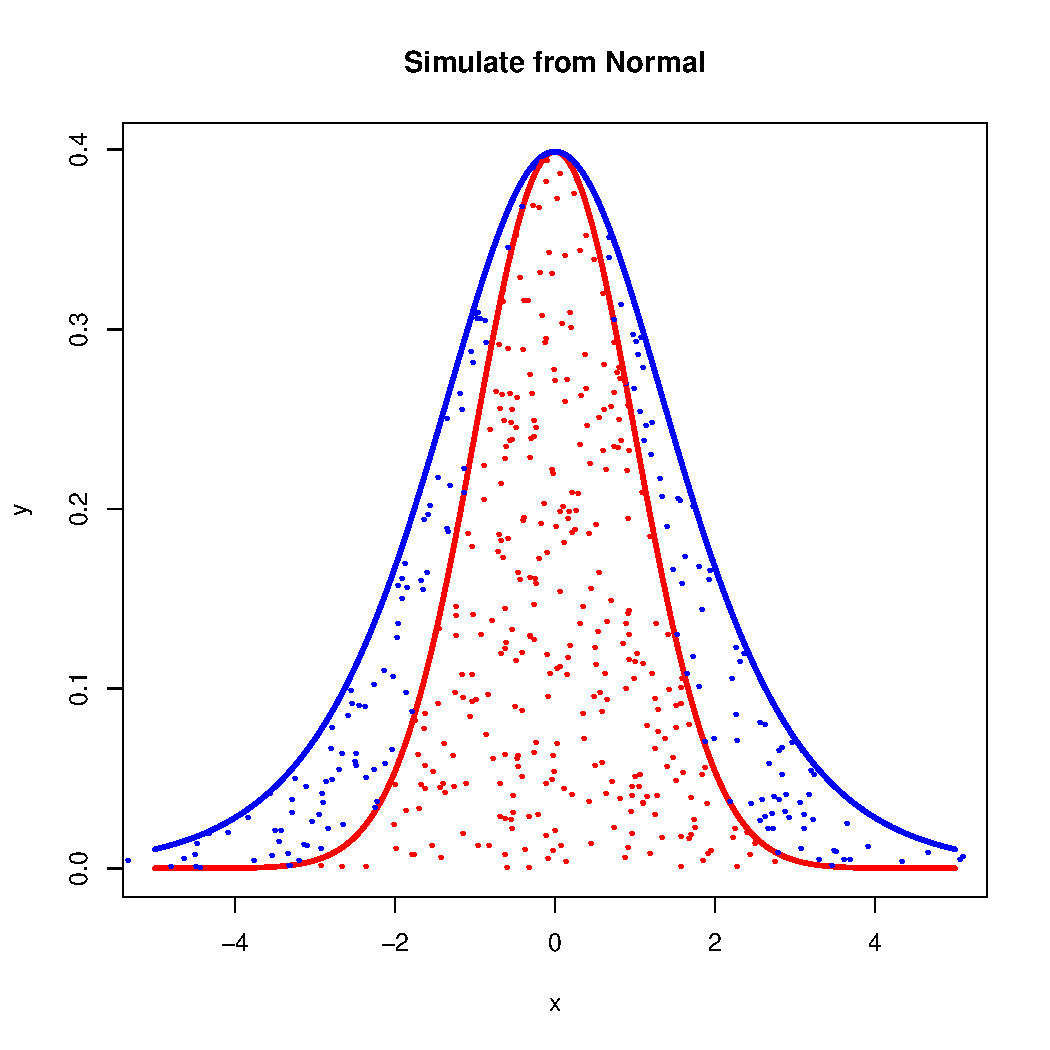
\includegraphics[height=7cm]{./Pics/nmlg3.pdf}
\end{center}
\end{frame}
\begin{frame}{The idea}
\begin{itemize}
\item Let $p(x)$ be the {\bf target distribution} and $q(x)$ be the {\bf proposal distribution}
\pause
\item Simulate an $x$-coordinate from the proposal $q(x)$
\pause
\item Simulate a y-coordinate from $U(0,Mq(x))$
\pause
\item Reject any points that are not `inside' $p(x)$
\pause
\item In our example what is
\begin{itemize}
\item The target distribution (normal or logistic?)
\item The proposal distribution (normal or logistic?)
\end{itemize}
\end{itemize}
\end{frame}
\begin{frame}{The Accept/Reject algorithm}
\begin{enumerate}
\item Simulate $x\sim q(x)$ 
\item Simulate $y\sim U(0,1)$. If \alt{$y<\frac{p(x)}{q(x)M}$}{$Mq(x)y<p(x)$}<2>
\begin{itemize}
\item Keep $x$ 
\end{itemize}
Otherwise
\begin{itemize}
\item Reject $x$ 
\end{itemize}
\end{enumerate}
The values of $x$ have density $p(x)$
\end{frame}
\begin{frame}{Accept/Reject Algorithm}
\begin{center}
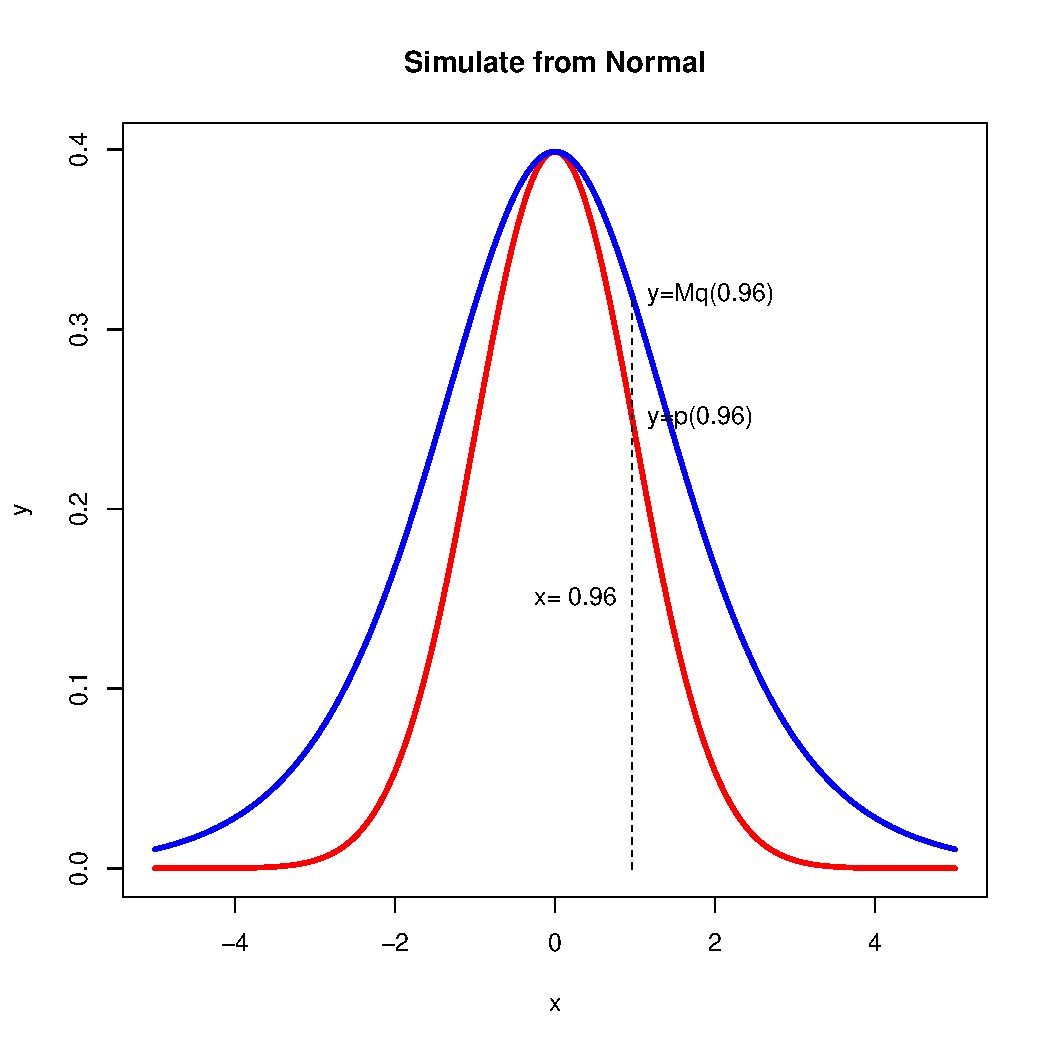
\includegraphics[height=7cm]{./Pics/nmlg4.pdf}
\end{center}
\end{frame}
\begin{frame}{Accept/Reject Algorithm}
\begin{center}
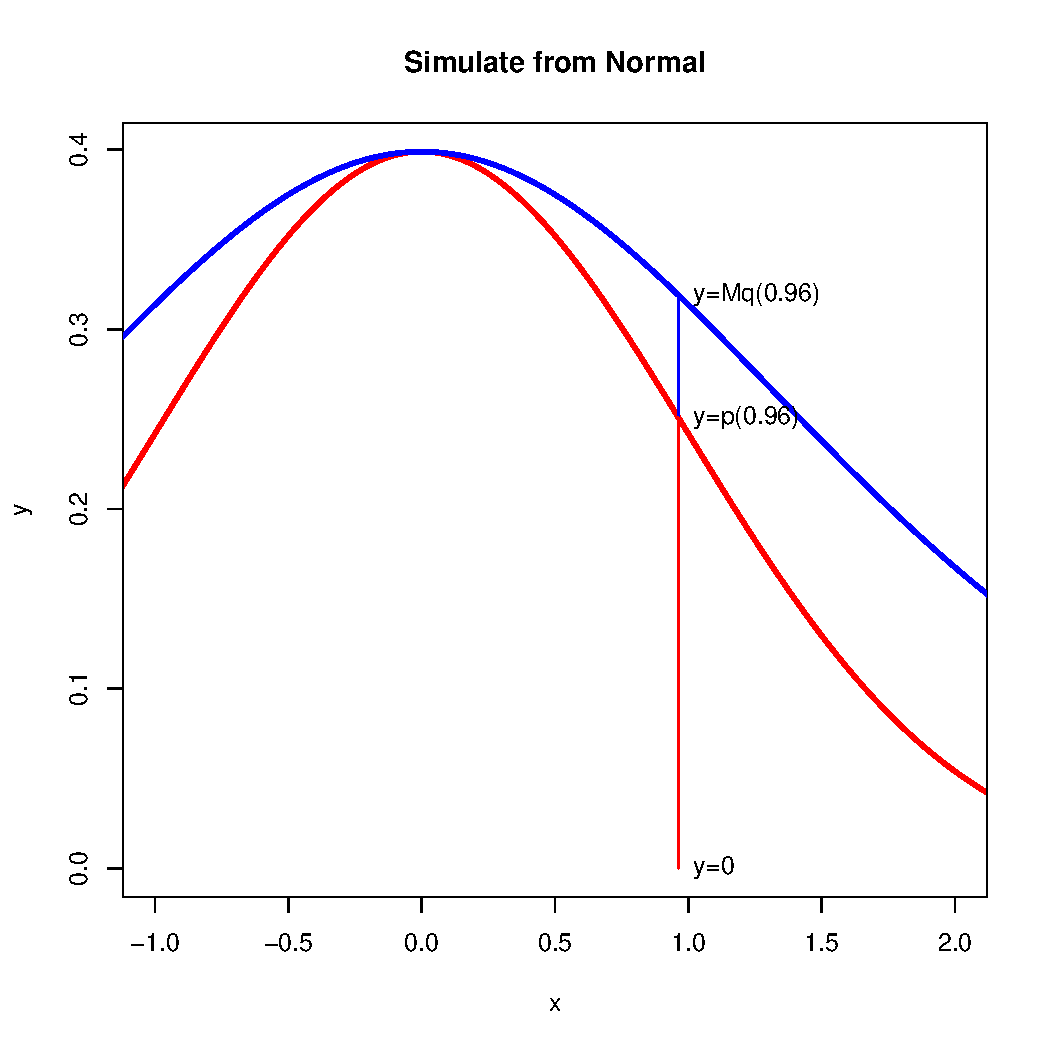
\includegraphics[height=7cm]{./Pics/nmlg5.pdf}
\end{center}
\end{frame}
\begin{frame}{Accept/Reject Algorithm}
\begin{center}
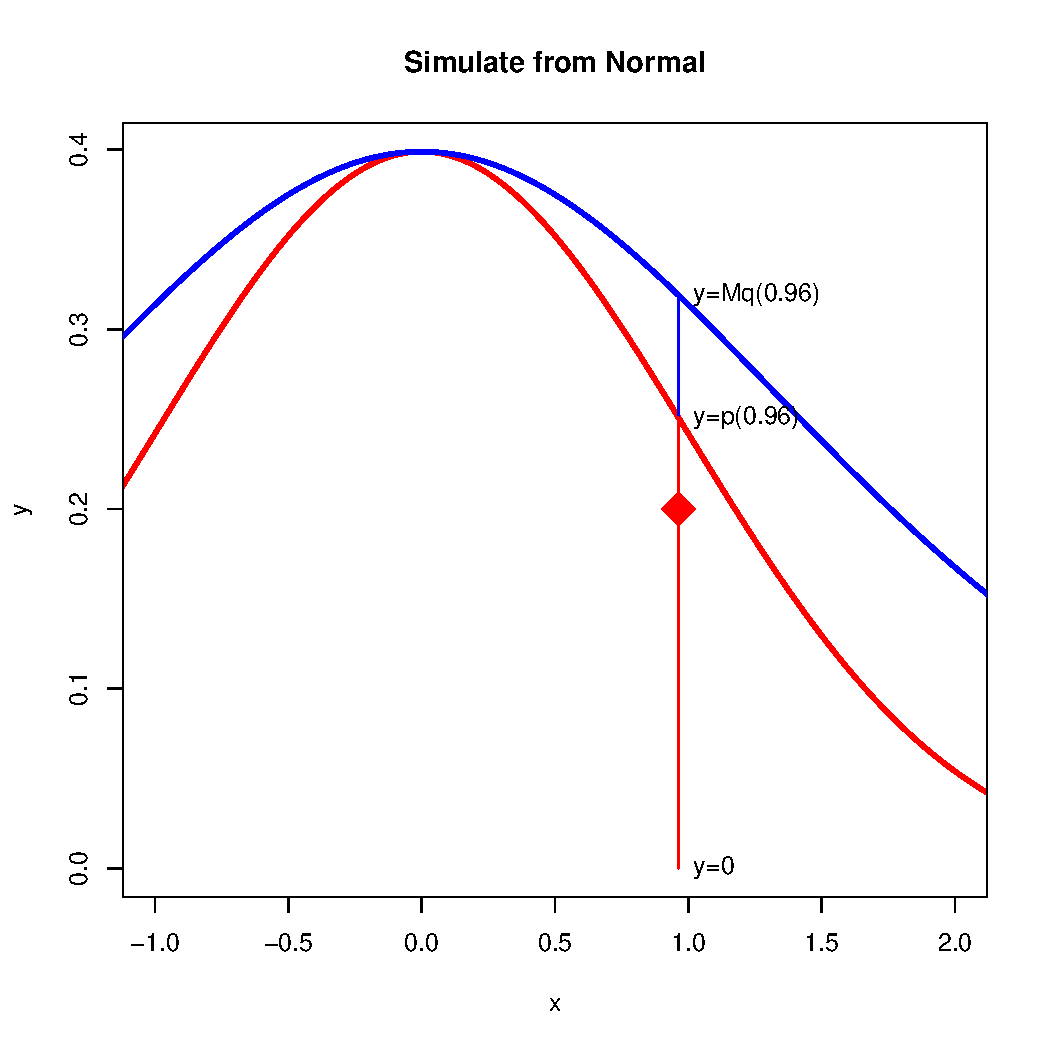
\includegraphics[height=7cm]{./Pics/nmlg6.pdf}
\end{center}
\end{frame}
\begin{frame}{Accept/Reject Algorithm}
\begin{center}
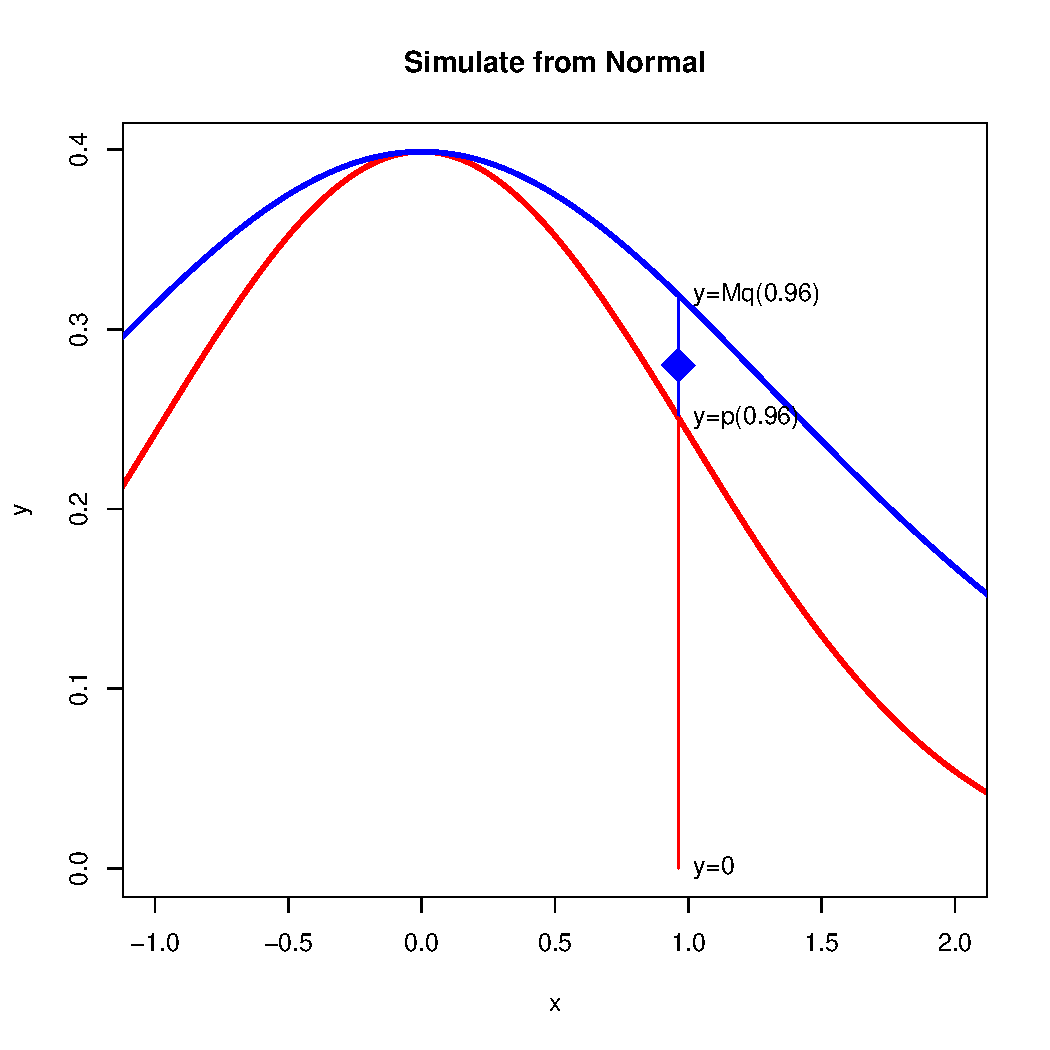
\includegraphics[height=7cm]{./Pics/nmlg7.pdf}
\end{center}
\end{frame}
\begin{frame}{Formal Proof}
Let $x\sim q(x)$ be accepted if $y<\frac{f(x)}{Mq(x)}$ where $y\sim U(0,1)$.  Also assume (without loss of generality) that $x\in\mathbb{R}$ 
\begin{align*}
\mbox{Pr}(x\leq x^*|\mbox{Accept})&=\frac{Pr\left(x\leq x^*,\mbox{Accept}\right)}{\mbox{Pr(Accept)}}\\
&=\frac{\mbox{Pr}\left(x\leq x^*,y<\frac{f(x)}{Mq(x)}
\right)}{\mbox{Pr}\left(y<\frac{f(x)}{Mq(x)}\right)}\\
&=\frac{\int_{-\infty}^{x^*}\int_{0}^{\frac{f(x)}{Mq(x)}}q(x)dydx}{\int_{-\infty}^{\infty}\int_{0}^{\frac{f(x)}{Mq(x)}}q(x)dydx}
\end{align*}
\end{frame}
\begin{frame}{Formal Proof}
\begin{align*}
\mbox{Pr}(x\leq x^*|\mbox{Accept})&=\frac{\int_{-\infty}^{x^*}\int_{0}^{\frac{f(x)}{Mq(x)}}dyq(x)dx}{\int_{-\infty}^{\infty}\int_{0}^{\frac{f(x)}{Mq(x)}}dyq(x)dx}\\
&=\frac{\int_{-\infty}^{x^*}\frac{f(x)}{Mq(x)}q(x)dx}{\int_{-\infty}^{\infty}\frac{f(x)}{Mq(x)}q(x)dx}\\
&=\frac{\frac{1}{M}\int_{-\infty}^{x^*}f(x)dx}{\frac{1}{M}\int_{-\infty}^{\infty}f(x)dx}\\
&=\int_{-\infty}^{x^*}f(x)dx
\end{align*}
\end{frame}
\begin{frame}{Choosing $q(x)$ and $M$}
\begin{itemize}
\item Two things are necessary for the accept/reject algorithm to work:
\pause
\begin{enumerate}
\item The domain of $p(x)$ and the domain of $q(x)$ MUST be the same.  
\item The value of $M$ must satisfy $M\geq \sup_x p(x)/q(x)$
\end{enumerate}
\end{itemize}
\end{frame}
\begin{frame}{Choosing $q(x)$ and $M$}
\begin{itemize}
\item The algorithm will be more {\bf efficient} if:
\pause
\begin{enumerate}
\item The proposal $q(x)$ is a good approximation to $p(x)$ 
\item The value of $M$ is $M=\sup_x p(x)/q(x)$
\end{enumerate}
\end{itemize}
\end{frame}
\begin{frame}{A look at $p(x)/q(x)$}
\begin{center}
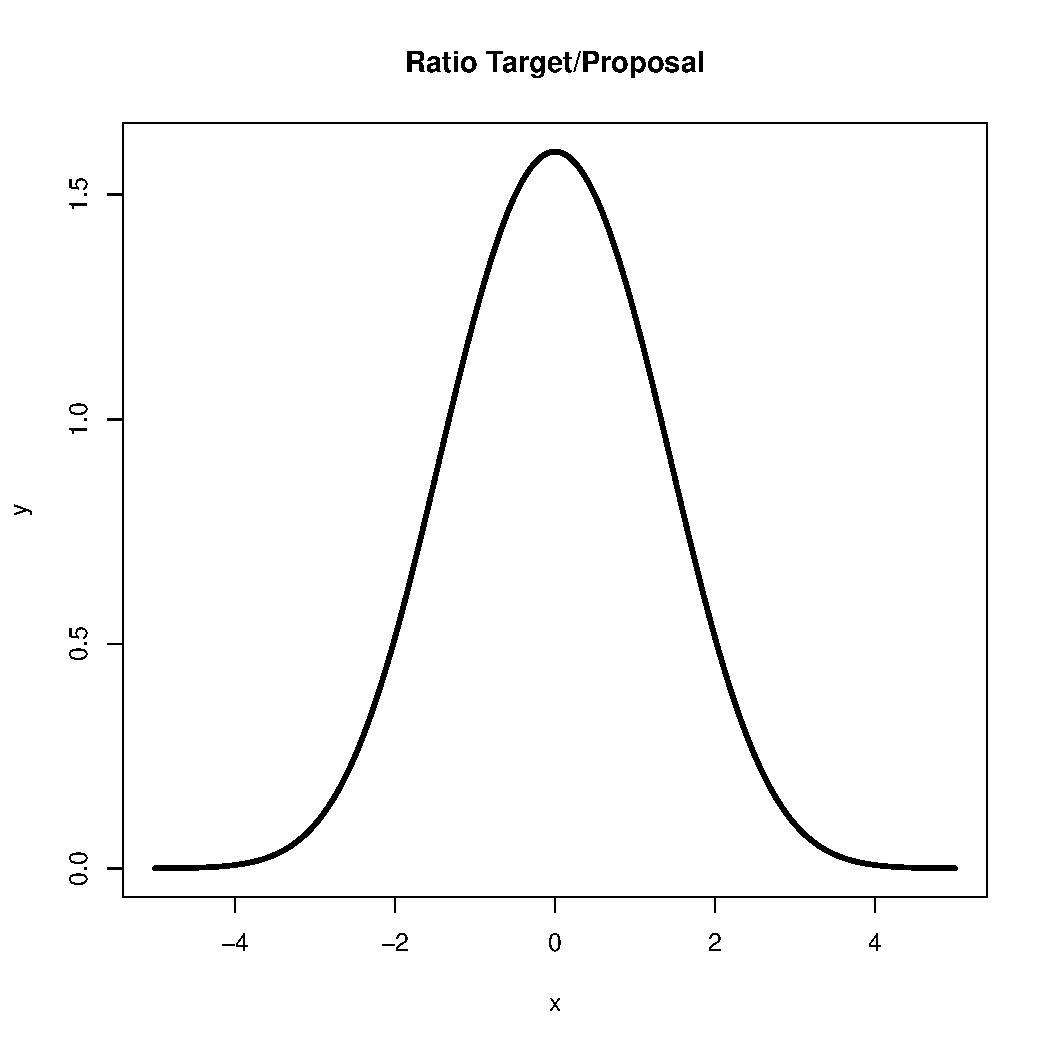
\includegraphics[height=7cm]{./Pics/rat1.pdf}
\end{center}
\end{frame}
\begin{frame}{Choosing $M$}
\begin{itemize}
\item From the plot one can see that the supremum of $p(x)/q(x)$ is at the point $x=0$
\pause
\item This gives an optimal value of $M=1.5958$
\pause
\item Suppose the problem is reversed.  Now the logistic is the target distribution and the normal is the proposal distribution.
\pause
\item Does this work?
\end{itemize}
\end{frame}
\begin{frame}{A look at $p(x)/q(x)$}
\begin{center}
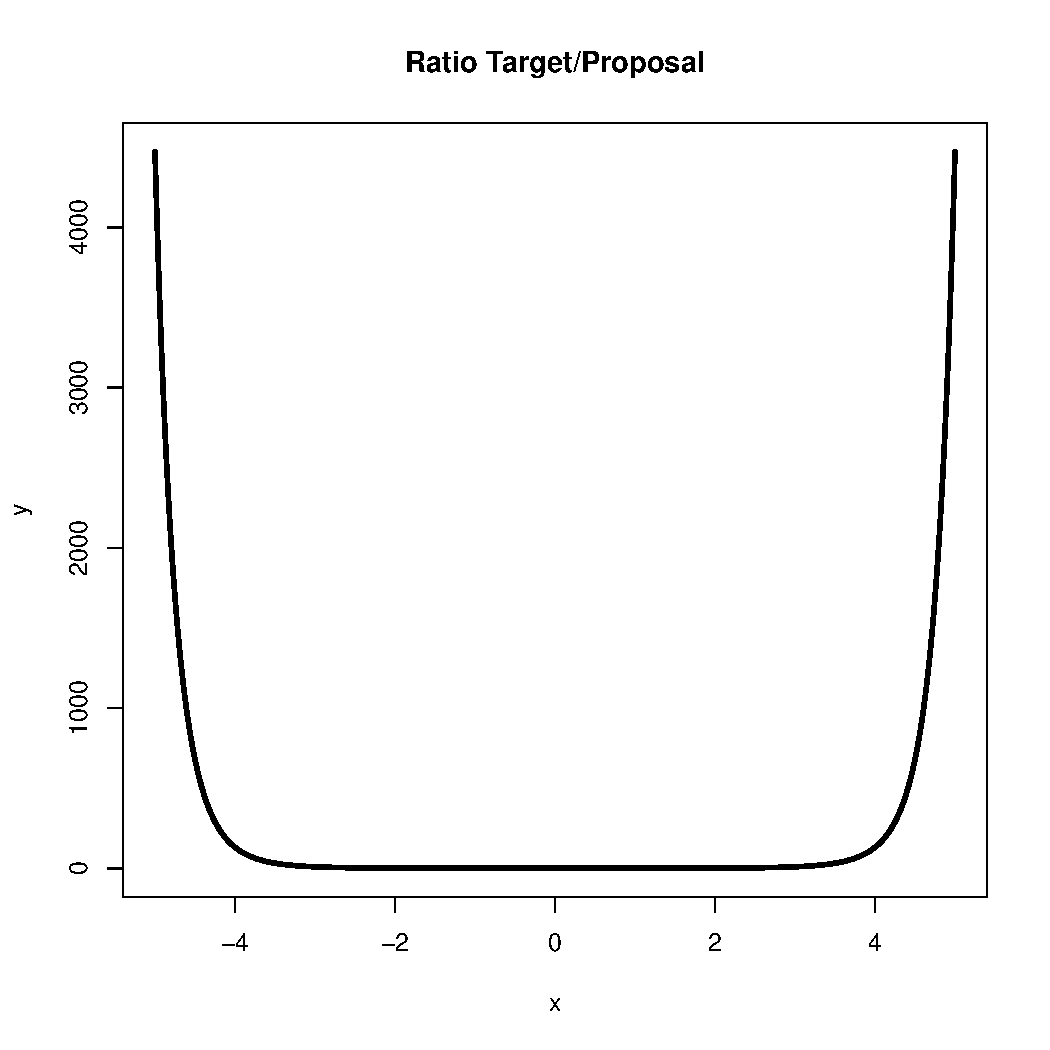
\includegraphics[height=7cm]{./Pics/rat2.pdf}
\end{center}
\end{frame}
\begin{frame}{Normalizing Constant and Kernel}
\begin{itemize}
\item Today we saw many density functions $f(x)$
\item Many density functions can written as $f(x)=k\tilde{f}(x)$
\item The part $k$ is called the
\alt<2>{{\color{blue} normalizing constant}}{ normalizing constant} 
and the part $\tilde{f}(x)$ is called the
\alt<2>{{\color{red} kernel}}{kernel}.
\item For example the standard normal distribution is
\alt<2>
{\begin{equation}
p(x)={\color{blue}(2\pi)^{-1/2}}{\color{red}e^{-x^2/2}}
\end{equation}}
{\begin{equation}
p(x)=(2\pi)^{-1/2}e^{-x^2/2}
\end{equation}} 
\pause
\end{itemize}
\end{frame}
\begin{frame}{Normalizing Constant and Kernel}
What are the 
\alt<1>{ normalizing constant}{{\color{blue} normalizing constant}} 
and 
\alt<1>{kernel}{{\color{red} kernel}} 
of the Beta function?
\alt<1>{
\begin{equation}
\mbox{Beta}(x;a,b)=\frac{\Gamma(a+b)}{(\Gamma(a)\Gamma(b))}x^{a-1}(1-x)^{b-1}
\end{equation}
}{
\begin{equation}
\mbox{Beta}(x;a,b)={\color{blue}\frac{\Gamma(a+b)}{(\Gamma(a)\Gamma(b))}}{\color{red}x^{a-1}(1-x)^{b-1}}
\end{equation}
}
\pause
\end{frame}
\begin{frame}{Accept/Reject and the normalising constant}
\begin{itemize}
\item An advantage of the Accept/Reject algorithm is that is works, even if the normalizing constant is unavailable.
\pause
\item Only the kernel is needed.
\pause
\item There are many examples where the normalising constant is either unavailable or difficult to compute.
\pause
\item This often happens in Bayesian analysis
\end{itemize}
\end{frame}
\begin{frame}{Summary}
\begin{itemize}
\item At the beginning of the day we only assumed that there was a way to simulate $U(0,1)$
\pause
\item Now we can simulate from many distributions:
\pause
\item Using the direct method if
\pause
\begin{itemize}
\item The inverse CDF can be computed
\end{itemize}
\pause
\item Using the indirect method if
\pause
\begin{itemize}
\item The density is available
\item A suitable proposal can be found
\end{itemize}
\pause
\item For the indirect method we do not even need the normalizing constant.
\pause
\item What about other methods?\pause Next week
\end{itemize}
\end{frame}
%\section{Indirect Simulation: Metropolis Algorithm}
%\subsection{Metropolis Algorithm}
%\begin{frame}{Markov chain}
%Markov chain
%\end{frame}
%\begin{frame}{Random Walk proposal}
%Markov chain
%\end{frame}
%\subsection{Metropolis Hastings Algorithm}
%\begin{frame}{Non-symmetric Proposal}
%Met Hastings
%\end{frame}
%\begin{frame}{Laplace Approximation}
%Laplace
%\end{frame}
%\subsection{Gibbs Sampler}
%\begin{frame}{Simulating more than one variable}
%Gibbs
%\end{frame}
\end{document}